\documentclass[book, 14pt]{memoir}
\usepackage[utf8]{inputenc}
\usepackage{hyperref}
%\usepackage{euler}
\usepackage{todo}
\usepackage{blindtext}
\usepackage{graphicx}
\usepackage{tabularx}
\usepackage{calc}
\usepackage{euler}
\usepackage{longtable}
\setlrmarginsandblock{3cm}{3cm}{*}
\setulmarginsandblock{3cm}{3cm}{*}
\checkandfixthelayout

%%%%%%%%%%%%%%%%%%%%% Telefon-Umgebung %%%%%%%%%%%%%%%%%%%%%
\newenvironment{telefon}[1]{%
	\par
	\noindent{\large \ding{38}}
	\begin{minipage}[t]{14.5cm}
		\textbf{Telefonat mit #1:}
		}{
	\end{minipage}
	\par
}

%%%%%%%%%%%%%%%%%%%%% E-Mail-Umgebung %%%%%%%%%%%%%%%%%%%%%
\newenvironment{mail}[1]{%
	\vspace{0.5em}
	\par
	\noindent{\large \ding{41}}
	\begin{minipage}[t]{14.5cm}
		\textbf{E-Mail an #1:}
		}{
	\end{minipage}
	\par
}

%%%%%%%%%%%%%%%%%%%%% Chat-Umgebung %%%%%%%%%%%%%%%%%%%%%
\newenvironment{chat}[1]{%
	\par
	\noindent{\large \copyright}
	\begin{minipage}[t]{14.5cm}
		\textbf{Chat mit #1:}
		}{
	\end{minipage}
	\par
}

%%%%%%%%%%%%%%%%%%%%% Gammeliese-Umgebung %%%%%%%%%%%%%%%%%%%%%
\newenvironment{gammeliese}[1]{%
	\vspace{0.5em}
	\par
	\noindent{\large \ding{41}}
	\begin{minipage}[t]{14.5cm}
		}{
	\end{minipage}
	\par
}
	
\begin{document}

%%%%%%%%%%%%%%%%%%%%% Aussehen Kapitel %%%%%%%%%%%%%%%%%%%%%
\providecommand{\HUGE}{\Huge}
\newlength{\drop}
\newcommand*{\FSfont}[1]{\fontencoding{T1}\fontfamily{#1}\selectfont}
\newcommand*{\TXfont}[1]{\fontencoding{T1}\fontfamily{#1}\selectfont}
\makeatletter
\DeclareRobustCommand\ltseries
{\not@math@alphabet\ltseries\relax
\fontseries\ltdefault\selectfont}
\newcommand{\ltdefault}{l}
\DeclareRobustCommand\hbseries
{\not@math@alphabet\hbseries\relax
\fontseries\hbdefault\selectfont}
\newcommand{\hbdefault}{hb}
\chapterstyle{chappell}

%%%%%%%%%%%%%%%%%%%%% Aussehen Titelseite %%%%%%%%%%%%%%%%%%%%%
\begin{minipage}[hbt]{5cm}
	\centering
	
\includegraphics[width=45mm]{logo_fokus}
\end{minipage}
\hfill
\begin{minipage}[hbt]{5cm}
	\centering
	
\includegraphics[width=50mm]{logo_fu-berlin}
\end{minipage}

\begin{center}
\thispagestyle{empty}
\drop=0.1\textheight
\settowidth{\unitlength}{\LARGE *************************************}
\vspace*{\baselineskip}\vspace*{\baselineskip}\vspace*{\baselineskip}
\vspace*{\baselineskip}\vspace*{\baselineskip}\vspace*{\baselineskip}
{\scshape Damla Durmaz, Ferhat Beyaz, Sebastian Barthel, Arsenij Solovjev, Markus Rudolph, Alexander Dümont}\\[\baselineskip]
\rule{\unitlength}{1.3pt}\\[\baselineskip]
{\LARGE Sonar Modelbus Plugin \\ Project Manual}\\[\baselineskip]
{\itshape Softwareproject WiSe 2012 \\ Modelbased Software Engineering Softwareentwicklung}\\[0.2\baselineskip]
\rule{\unitlength}{1.3pt}\\[\baselineskip]
{\large\scshape \today}\par
\vfill
%{\large\scshape \textrm{XIII} }\\[\baselineskip]
{\small\scshape \textrm{Freie Universität Berlin, Fachbereich Informatik \\ AG Software Engineering, Wintersemester 2012} \\ Ina Schieferdecker, Tom Ritter und Christian Hein}
\par\vspace*{\drop}
\end{center}
\clearpage

%%%%%%%%%%%%%%%%%%%%% KAPITEL %%%%%%%%%%%%%%%%%%%%%
\tableofcontents
\chapter{Introduction}

\section{Motivation}
Sonar (\autoref{sec:sonar}) is an open source software quality platform that uses various static code analysis tools such as Checkstyle, PMD and FindBugs to extract software metrics, which can be used to improve software quality. For source code, Sonar can even give comments on analyzed code, such as what kind of major bugs are found or conventions are not hold and what can be done to resolve it. Usually, Sonar is used in combination with programming languages, like Java, C or C\#, but Sonar indeed gives the functionality to display all kind of measures and handle more than just source code. From model driven software development (\autoref{sec:model_driven_engineering}) we know, that all the object oriented ideas also can be mapped to models, which represent the original objects. So in fact, we also could analyze models instead of just source code. This aspect can be very useful in enterprises, which only work model driven. Instead of transforming their models into source code, they can only rely on the standards, given for the used model language, and can analyze their models with Sonar. This has a great advantage: Instead of firstly generating code from their models and then analyzing their source code by Sonar, they simply can use the models only, analyze them with Sonar and only when the measurements reached a specified threshold, they can generate code from their models. Thus, developers can evaluate, change and improve code quality before generating code. 

Within the \textit{Softwareprojekt modellgetriebene Softwareentwicklung} at \textit{Freie Universit\"at Berlin}, we worked together with \textit{Frauenhofer FOKUS}, an institution of \textit{Frauenhofer Gesellschaft}. The corresponding \textit{Fraunhofer-Institut für Offene Kommunikationssysteme} has a technology, called Modelbus (\autoref{sec:modelbus}), a modelling framework with a model repository behind, which is used to achieve a seamless integration between tools and the work of the development team. In Modelbus, system information (models) can be stored and reused in a transparent way. The idea is to combine the work of Sonar with the work of Modelbus: Models from the Modelbus repository can be fetched, analyzed and the results can be visualized to the developer.

Sonar metrics are metrics for normal source code. But there are a lot of Sonar metrics, which can be transferred logically to metrics for object oriented models, for example UML models. Therefore, Sonar metrics must be translated into object oriented metrics, which can be applied to models from the Modelbus repository. Since we cannot simply use all of the metrics we know from object oriented code analysis, Sonar cannot be run out of the box to analyze models. Our plugin should therefore use the Metrino service (\autoref{sec:metrino}), which gives us the functionality to examine all of the metrics on models as well. So with our work we want to provide a Sonar plugin to analyze models located at a Modelbus repository using the Metrino Service.

\section{Model-Driven Engineering} \label{sec:model_driven_engineering}
With model-driven engineering we focus on domain models rather then on objects in the sense of object oriented programming. Those domain models are anbstract representations of the knowledge and activities that belong them). We can compare them with objects, but instead of describing them with sourcecode from programming languages like Java or C we simply use UML and generate the sourcecode from it.

With the usage of standardized models model-driven engineering wants to maximize the compatibility between systems and wants to increase the overall productivity. Models are developed in the communication process between the product owner, developers and other people (designers, etc). As the model set approaches completion, development process can be started.

\section{Expectations}
Our team consists of six computer science MSc students who are motivated to find a stable solution for the given task: Alexander Dümont, Arsenij Solovjev, Damla Durmaz, Ferhat Beyaz, Markus Rudolph and Sebastian Barthel.

Our goal is to expand Sonar to cooperate with Modelbus. At the beginning of the course, none of us had experience in working with neither Sonar nor Modelbus nor Metrino. So, in fact our first expectation was to learn the usage of those software systems. We also had not much experience in the model driven software developement. Therefore it should be necessary to learn to work with models and to generate code from it (as later used within the SMM parser and other software components). Although we had no experience with those systems, their good programming interfaces are promising to work fluently together.

\section{Goal of this document}
The goal of this document is mainly to provide an overview of our Sonar plugin and its architecture. In \autoref{sec:sonar_modelbus_plungin}, the used technologies for our plugin are explained briefly. Firstly, Modelbus and the Metrino service are presented. Additionally, Sonar is presented and how a Sonar plugin can be developed in general. Afterward, the architecture of our software is shown and which formats are used to communicate with the Metrino service. Finally, we want to present a problem, which raised during the development and how it can be solved. In \autoref{sec:installation_usage}, an installation manual is provided and how the plugin can be used and especially, system requirements are mentioned. In the last chapter, the work will be reviewed and a conclusion is made. In the appendix (\autoref{sec:appendix}), we included our meeting protocols, which we made during each lecturer and other team meetings. These meeting protocols explain in detail our progress for each work, the problems, with which we were confronted and how the software progressed.

\section{Requirements}
The product owner presented us their system with Modelbus and the Metrino service. They explained, that in the Modelbus repository, there are models which can be analyzed by the Metrino service and that it can be interesting to get to know in what extend object oriented metrics of Sonar can be applied to models. Therefore, we identified some requirements for our Sonar plugin:
\begin{enumerate}
\item Create a plugin for sonar 
\item Comprehend and cooperate with ModelBus repository
\item Transfer as many as possible metrics from Metrino to Sonar
\item Select the model
\item Traverse the directory tree
\item Analyze source codes
\item Plugin must work as efficient as possible
\end{enumerate}
In the following sections, the requirements will be described in detail and are divided into functional and non-functional requirements.

\subsection{Functional requirements}

\begin{table}[H]
\begin{tabular}{|c|p{10cm}|}
\hline 
\multicolumn{2}{|l|}{\textbf{Create a plugin for Sonar}} \\ 
\hline 
Requirement Number & 1 \\ \hline 
Description & Each sonar plugin has a specific architecture. The created sonar plugin must hold the specifications for a sonar plugin. Additionally, it must be run on a server and offers a WSDL interface. \\ \hline 
Dependencies & \textbf{none} (should be done first) \\ \hline 
Priority & high \\ \hline 
State & closed \\ \hline 
Fit Criterion & The plugin can be build and runs on a chosen server. A client connects to the Modelbus server and understands the WSDL interface. The client receives a message from the WSDL interface of the Modelbus server. \\ \hline 
\end{tabular}
\end{table}

\begin{table}[H]
\begin{tabular}{|c|p{10cm}|}
\hline 
\multicolumn{2}{|l|}{\textbf{Comprehend and cooperate with ModelBus repository}} \\ 
\hline 
Requirement Number & 2 \\ \hline 
Description & ModelBus has an own repository, where it stores artifacts of the tools, which are connected to the ModelBus via adapters. It must be understood, how ModelBus connects to the repository and how an external tool (like a sonar plugin) can do this. \\ \hline 
Dependencies & \# 1 \\ \hline 
Priority & high \\ \hline 
State & closed \\ \hline 
Fit Criterion & The sonar plugin is able to connect to the ModelBus repository via a command. It can fetch the source code for a random project to test, if the connection is established. The sonar plugin can terminate the connection to the repository for a given command. \\ \hline 
\end{tabular}
\end{table}

\begin{table}[H]
\begin{tabular}{|c|p{10cm}|}
\hline 
\multicolumn{2}{|l|}{\textbf{Select the model}} \\ 
\hline 
Requirement Number & 4 \\ \hline 
Description & The sonar plugin can fetch model code from the repository and transform the model into a format which can be read by model metric analyzing tools, like Metrino. \\ \hline 
Dependencies & \# 3 \\ \hline 
Priority & high \\ \hline 
State & closed \\ \hline 
Fit Criterion & The plugin fetched a model. It transforms the model into the format of Metrino. For a test case, the transformed model shall be saved in a file and read successfully by Metrino. \\ \hline 
\end{tabular}
\end{table}
\vspace{-30mm}
\begin{table}[H]
\begin{tabular}{|c|p{10cm}|}
\hline 
\multicolumn{2}{|l|}{\textbf{Traverse the directory tree}} \\ 
\hline 
Requirement Number & 5 \\ \hline 
Description & In the directory tree of sonar plugin, a lot of source code and model code projects are placed. The plugin should be able to analyze all codes from the repository. \\ \hline 
Dependencies & \textbf{none} \\ \hline 
Priority & high \\ \hline 
State & closed \\ \hline 
Fit Criterion & The plugin fetched the whole project tree of the repository. It loads each project into its own directory tree. It traverses the whole directory tree. For each project in its directory tree, it analyzes the code and visualizes it on the web interface. \\ \hline 
\end{tabular}
\end{table}

\noindent\begin{minipage}{\linewidth}
\centering
\begin{tabular}{|c|p{10cm}|}
\hline 
\multicolumn{2}{|l|}{\textbf{Analyze source codes}} \\ 
\hline 
Requirement Number & 6 \\ \hline 
Description & The sonar plugin can apply a set of metrics to the fetched source code. The results are visualized with graphs or statistics and can be get via the web interface. \\ \hline 
Dependencies & \# 2 \\ \hline 
Priority & high \\ \hline 
State & Canceled, because requirement is unfeasible with current Sonar version (could be with future versions) \\ \hline 
Fit Criterion & The plugin fetches source code from the repository. It applies a couple of metrics, which can be chosen from the application interface. \\ \hline 
\end{tabular}
\end{minipage}

\subsection{Non-functional requirements}

\noindent\begin{minipage}{\linewidth}
\centering
\begin{tabular}{|c|p{10cm}|}
\hline 
\multicolumn{2}{|l|}{\textbf{Transfer as many as possible metrics from Metrino to Sonar}} \\ 
\hline 
Requirement Number & 3 \\ \hline 
Description & The sonar plugin can already fetch model code from the repository. The models are read by Metrino and analyzed by Metrino with object oriented metrics. The results of the analysis are fetched from Metrino by the sonar plugin and visualized on the web interface. Metrino offers a lot of metrics and it should be possible to offer as many metrics from Metrino as possible. \\ \hline 
Dependencies & \# 4 \\ \hline 
Priority & high \\ \hline 
State & open \\ \hline 
Fit Criterion & The sonar plugin sends a model to Metrino with the information which object oriented metric shall be applied. Metrino returns the results. The results are visualized. The plugin offers to select at least $10$ object oriented metrics of Metrino to apply to the sent model code. \\ \hline 
\end{tabular}
\end{minipage}

\noindent\begin{minipage}{\linewidth}
\centering
\begin{tabular}{|c|p{10cm}|}
\hline 
\multicolumn{2}{|l|}{\textbf{Plugin must work as efficient as possible}} \\ 
\hline 
Requirement Number & 7 \\ \hline 
Description & Plugin must traverse the directory tree fastly. The connection to the ModelBus must provide security standards, but it should not be slow. The results of the analysis should be offerred via the web interface as fast as possible. \\ \hline 
Dependencies & \# 6 \\ \hline 
Priority & middle \\ \hline 
State & closed \\ \hline 
Fit Criterion & Because of the difficulty of the decision, if it works properly fast, a usability test with the customer must be done, who can tell in a better way, if the product works fast or not. \\ \hline 
\end{tabular}
\end{minipage}



\section{Responsibilities and Progress}
\begin{table}[htbp]
  \caption{Exercises pt. 1}
  \noindent\hspace*{-1cm}\begin{tabularx}{\textwidth+2cm}{
>{\raggedleft\arraybackslash\advance\hsize1em}X
>{\raggedright\arraybackslash\advance\hsize1em }X
>{\raggedright\arraybackslash}X
>{\raggedright\arraybackslash\advance\hsize-1em }X
>{\raggedright\arraybackslash\advance\hsize-1em }X
}
    \addlinespace
    \toprule
    \multicolumn{1}{c}{Exercise } & Begin & End  & Progress & Done by   \\
    \midrule
         
        Explore Modelbus & Mo 05.11.12 & Fr 09.11.12 & 100\% & Team \\
Explore Sonar                                                           & Mo 05.11.12 & Fr 09.11.12 & 100\%     & Team                    \\ 
        Explore plugin developement possibilities                               & Mo 05.11.12 & Fr 09.11.12 & 100\%     & Ferhat                  \\ 
        Explore Sonar features and developement possibilities                   & Mo 05.11.12 & Fr 09.11.12 & 100\%     & Damla                   \\ 
        First attempt to plugin developement                                    & Mo 05.11.12 & Fr 09.11.12 & 100\%     & Markus                  \\ 
        Wiki Introduction                                                       & Mo 05.11.12 & Fr 09.11.12 & 100\%     & Sebastian               \\ 
        Modelbus connection                                                     & Mo 05.11.12 & Fr 09.11.12 & 100\%     & Arsenij                 \\ 
        Sonar documentation                                                     & Mo 05.11.12 & Fr 09.11.12 & 100\%     & Markus                  \\ 
        Wiki Metrino                                                            & Mo 05.11.12 & Fr 09.11.12 & 100\%     & Alexander               \\ 
        Sonar plugin documentation                                              & Mo 05.11.12 & Fr 09.11.12 & 100\%     & Ferhat                  \\ 
        Modelbus documentation                                                  & Mo 05.11.12 & Fr 09.11.12 & 100\%     & Damla                   \\ 
        Requirements                                                            & Mo 05.11.12 & Fr 09.11.12 & 100\%     & Damla  \&  Ferhat       \\ 
        Presentation Requirements                                               & Mo 05.11.12 & Fr 09.11.12 & 100\%     & Ferhat                  \\ 
        Improve requirements                                                    & Mo 12.11.12 & Fr 16.11.12 & 100\%     & Damla                   \\ 
        \hline
    \end{tabularx}\hspace*{-1cm}%
  \label{tab:addlabel}%
\end{table}%

\begin{table}[htbp]
  \caption{Exercises pt. 2}
  \noindent\hspace*{-1cm}\begin{tabularx}{\textwidth+2cm}{
>{\raggedleft\arraybackslash\advance\hsize1em}X
>{\raggedright\arraybackslash\advance\hsize1em }X
>{\raggedright\arraybackslash}X
>{\raggedright\arraybackslash\advance\hsize-1em }X
>{\raggedright\arraybackslash\advance\hsize-1em }X
}
    \addlinespace
    \toprule
    \multicolumn{1}{c}{Exercise } & Begin & End  & Progress & Done by   \\
    \midrule
        Architecture conecept for sonar                                         & Mo 12.11.12 & Fr 16.11.12 & 100\%     & Ferhat                  \\ 
        Architecture conecept for metrino                                       & Mo 12.11.12 & Fr 16.11.12 & 100\%     & Alexander               \\ 
        Introduction to wiki                                                    & Mo 12.11.12 & Mo 19.11.12 & 100\%     & Sebastian               \\ 
        Presentation Template                                                   & Mo 12.11.12 & Fr 19.11.12 & 100\%     & Damla                   \\ 
        Software architecture – sequencediagram/activitydiagram                 & Mo 12.11.12 & Fr 23.11.12 & 100\%     & Sebastian               \\ 
        Setup Modelbus Repository Server                                        & Mo 19.11.12 & Mo 26.11.12 & 100\%     & Arsenij                 \\ 
        Explore howto running sonar on a repository                             & Di 20.11.12 & Mo 26.11.12 & 100\%     & Arsenij                 \\ 
        Installation of software components                                     & Do 23.11.12 & Do 23.11.12 & 100\%     & Team                    \\ 
        Example Sonar plugin                                                    & Mo 19.11.12 & Fr 23.11.12 & 100\%     & Unknown                 \\ 
        Multilanguage (different programming languages) support in sonar plugins & Fr 23.11.12 & Do 29.11.12 & 100\%     & Markus  \&  Damla  \&  Ferhat \\ 

        \hline
    \end{tabularx}\hspace*{-1cm}%
  \label{tab:addlabel}%
\end{table}%

\begin{table}[htbp]
  \caption{Exercises pt. 3}
  \noindent\hspace*{-1cm}\begin{tabularx}{\textwidth+2cm}{
>{\raggedleft\arraybackslash\advance\hsize1em}X
>{\raggedright\arraybackslash\advance\hsize1em }X
>{\raggedright\arraybackslash}X
>{\raggedright\arraybackslash\advance\hsize-1em }X
>{\raggedright\arraybackslash\advance\hsize-1em }X
}
    \addlinespace
    \toprule
    \multicolumn{1}{c}{Exercise } & Begin & End  & Progress & Done by   \\
    \midrule
        Sequence diagram for the work of sonar with Metrino and ModelBus        & So 25.11.12 & So 25.11.12 & 100\%     & Damla  \&  Sebastian    \\ 
        Setup modelbus server                                                   & Fr 23.11.12 & Mo 26.11.12 & 100\%     & Markus                  \\ 
        Presentation first architecture                                         & Fr 23.11.12 & Mo 26.11.12 & 100\%     & Ferhat                  \\ 
        Activity diagram modelbus repository                                    & Fr 23.11.12 & Mo 26.11.12 & 100\%     & Damla                   \\ 
        SOAP Client Metrino                                                     & Fr 23.11.12 & Do 06.12.12 & 100\%     & Alexander               \\ 
        Wiki Logo and header                                                    & Mo 26.11.12 & Fr 30.11.12 & 100\%     & Ferhat                  \\ 
        OCL  \&  Documentation                                                  & Mo 26.11.12 & Fr 30.11.12 & 100\%     & Damla  \&  Ferhat       \\ 
        Milestone definitions and description                                   & Mo 26.11.12 & Fr 30.11.12 & 100\%     & Sebastian               \\ 
        Installation manual                                                     & Mo 03.12.12 & Mo 10.12.12 & 100\%     & Sebastian               \\ 
        Include other language plugins with modules                             & Mo 03.12.12 & Mo 10.12.12 & 100\%     & Arsenij                 \\ 
        \hline
    \end{tabularx}\hspace*{-1cm}%
  \label{tab:addlabel}%
\end{table}%


\begin{table}[htbp]
  \caption{Exercises pt. 4}
  \noindent\hspace*{-1cm}\begin{tabularx}{\textwidth+2cm}{
>{\raggedleft\arraybackslash\advance\hsize1em}X
>{\raggedright\arraybackslash\advance\hsize1em }X
>{\raggedright\arraybackslash}X
>{\raggedright\arraybackslash\advance\hsize-1em }X
>{\raggedright\arraybackslash\advance\hsize-1em }X
}
    \addlinespace
    \toprule
    \multicolumn{1}{c}{Exercise } & Begin & End  & Progress & Done by   \\
    \midrule
        Client without using WSDL by hand                                       & Mo 03.12.12 & Mo 10.12.12 & 100\%     & Markus                  \\ 
        Objectoriented Analysis to Models                                       & Mo 03.12.12 & Mo 10.12.12 & 100\%     & Ferhat                  \\ 
        Understand Metrino metrcis                                              & Mo 10.12.12 & Fr 21.12.12 & 100\%     & Sebastian  \&  Alexander \\ 
        ownload modelbus files in a sonar plugin                                & Mo 10.12.12 & Fr 21.12.12 & 100\%     & Markus                  \\ 
        Create latex documentation                                              & Mo 17.12.12 & Fr 21.12.12 & 100\%     & Ferhat                  \\ 
        Meeting Protocols to latex documentation                                & Mo 17.12.12 & Fr 21.12.12 & 100\%     & Damla                   \\ 
        Metrino CheckModel, download and parse SMM from Repo                    & Mo 07.01.13 & Mo 21.01.13 & 100\%     & Arsenij                 \\ 
        Sonar frontend                                                          & Mo 07.01.13 & Mo 21.01.13 & 100\%     & Sebastian               \\ 
        Parser for SMM                                                          & Mo 14.01.13 & So 20.01.13 & 100\%     & Damla  \&  Ferhat       \\ 
        Using of EMF to parse SMM files                                         & Mo 21.01.13 & Mo 28.01.13 & 100\%     & Damla  \&  Ferhat       \\ 

        \hline
    \end{tabularx}\hspace*{-1cm}%
  \label{tab:addlabel}%
\end{table}%


\begin{table}[htbp]
  \caption{Exercises pt. 5}
  \noindent\hspace*{-1cm}\begin{tabularx}{\textwidth+2cm}{
>{\raggedleft\arraybackslash\advance\hsize1em}X
>{\raggedright\arraybackslash\advance\hsize1em }X
>{\raggedright\arraybackslash}X
>{\raggedright\arraybackslash\advance\hsize-1em }X
>{\raggedright\arraybackslash\advance\hsize-1em }X
}
    \addlinespace
    \toprule
    \multicolumn{1}{c}{Exercise } & Begin & End  & Progress & Done by   \\
    \midrule
        Include parser into project workflow                                    & Mo 21.01.13 & Mo 28.01.13 & 100\%     & Damla  \&  Ferhat       \\ 
        Merge all components into one                                           & Mo 21.01.13 & Mo 28.01.13 & 100\%     & Arsenij                 \\ 
        Project spezific measurements in sonar                                  & Mo 21.01.13 & Mo 28.01.13 & 100\%     & Markus                  \\ 
        ceate ocl metrics                                                       & Mo 21.01.13 & So 03.02.13 & 100\%     & Alexander               \\ 
        Color Measurements                                                      & Mo 21.01.13 & Mo 28.01.13 & 100\%     & Sebastian               \\ 
        Documentation in Latex                                                  & Mo 28.01.13 & Mo 18.02.13 & 25\%      & Team                    \\ 
        SMM Adapter                                                             & Mo 28.01.13 & Mo 18.02.13 & 67\%      & Arsenij                 \\ 
        Load dynamic metrics in sonar                                           & Mo 28.01.13 & Mo 18.02.13 & 36\%      & Sebastian               \\ 
        Meeting Protocols                                                       & Mo 03.12.12 & Mo 18.02.13 & 95\%      & Damla  \&  Ferhat       \\
        
        \hline
    \end{tabularx}\hspace*{-1cm}%
  \label{tab:addlabel}%
\end{table}%

\newpage

\begin{figure}[htb]
\begin{center}
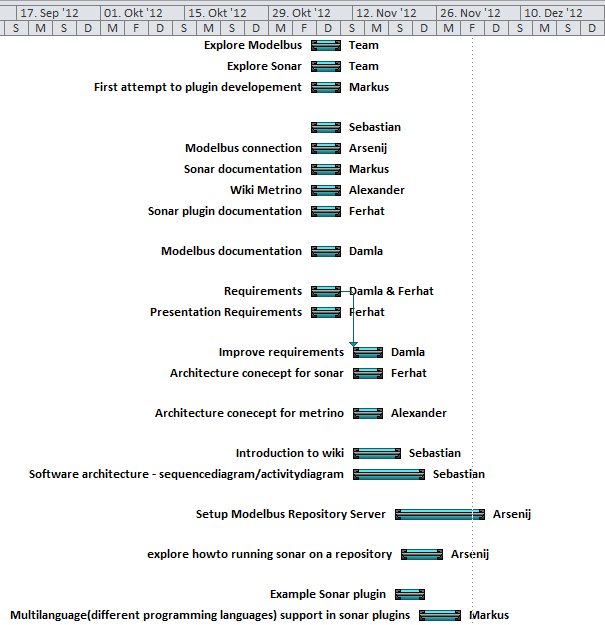
\includegraphics[width=\textwidth]{msp_part1}
\caption{Exercises - MS Project screenshot 1}
\end{center}
\end{figure}

\newpage

\begin{figure}[htb]
\begin{center}
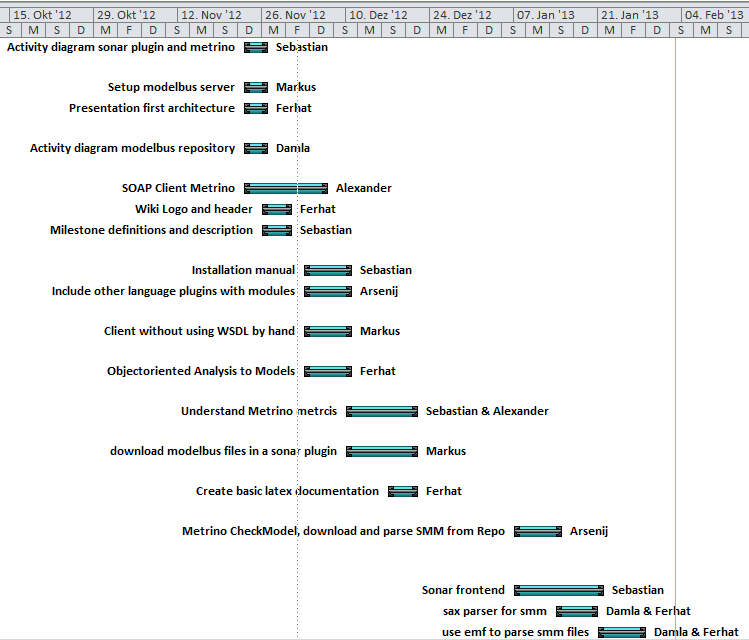
\includegraphics[width=\textwidth]{msp_part2}
\caption{Exercises - MS Project screenshot 2}
\end{center}
\end{figure}

\newpage

\begin{figure}[htb]
\begin{center}
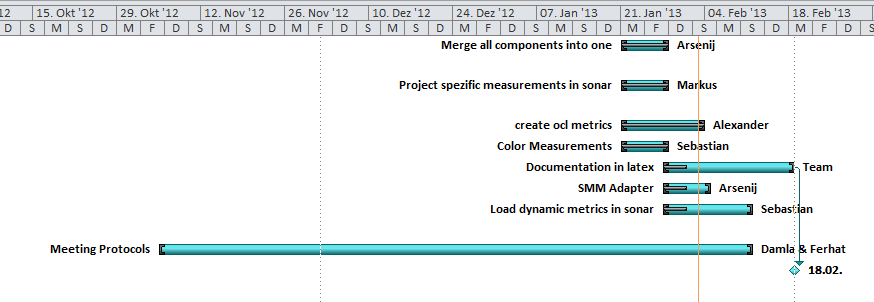
\includegraphics[width=\textwidth]{msp_part3}
\caption{Exercises - MS Project screenshot 3}
\end{center}
\end{figure}
\chapter{Installation and Usage}
\section{Software Requirements}
For development following software components are needed:

\begin{itemize}
	\item Java (JDK) 1.6 or 1.7
	\item Maven
  \item Eclipse (Juno)
	\item Maven Plugin for Eclipse
  \item Git or Egit for Eclipse
  \item Modelbus Team Provider for Eclipse
	\item Modelbus 1.9.7
	\item Metrino for Modelbus with following plugins
		\begin{itemize}
			\item Metrino rule evaluator plugin
			\item Metrino measure plugin
		\end{itemize}
\end{itemize}
Sonar will be downloaded and deployed via Maven at compile time.

\section{Installation Manual}
In the following sections we explain every detail. Just skip a section if you think you still have done that what the regarding section focuses. 

\subsection{Java}
We tested the software with Java 1.6 and 1.7. You can get those from \href{http://www.oracle.com/technetwork/java/javase/downloads/index.html}{here}. Select and download the current JDK to install it on your system. If Java is ready, make sure that the following system variables exist:
\begin{verbatim}
JAVA_HOME = C:\Program Files\Java\jdk1.7.0_09
(change the path to your JDK install path)
\end{verbatim}

Also you must add your JAVA\_HOME variable (add \textbackslash bin\textbackslash ) to your path variable.
\begin{verbatim}
PATH =...;%JAVA_HOME%\bin\;
\end{verbatim}

\subsection{Maven}
Download the current Maven from \href{http://maven.apache.org/download.html}{here} and follow the instructions from the README: Extract it somewhere and create following path variables:
\begin{verbatim}
M2_HOME = C:\Program Files\apache-maven-3.0.4 
(change the path to your maven folder)
M2 = %M2_HOME%\bin\
PATH =...;%M2%;
\end{verbatim}



\subsection{Eclipse}
Download Eclipse from \href{http://www.eclipse.org/juno/}{here}.
We recommend a current Eclipse version. We use Eclipse Juno (4.2) for Java developer.
Remember to select the correct version for your operating system. 



\subsection{Maven Plugin for Eclipse}
Open Eclipse and open "Help | Install New Software...". Now select or add the repository of your eclipse version. In our example we will use 

\url{http://download.eclipse.org/releases/juno}
 
Select "m2e – Maven Integration for Eclipse" and click through the progress to install the plugin. If everything works well, Eclipse will ask you for an Eclipse restart. 

\begin{figure}
	\centering
		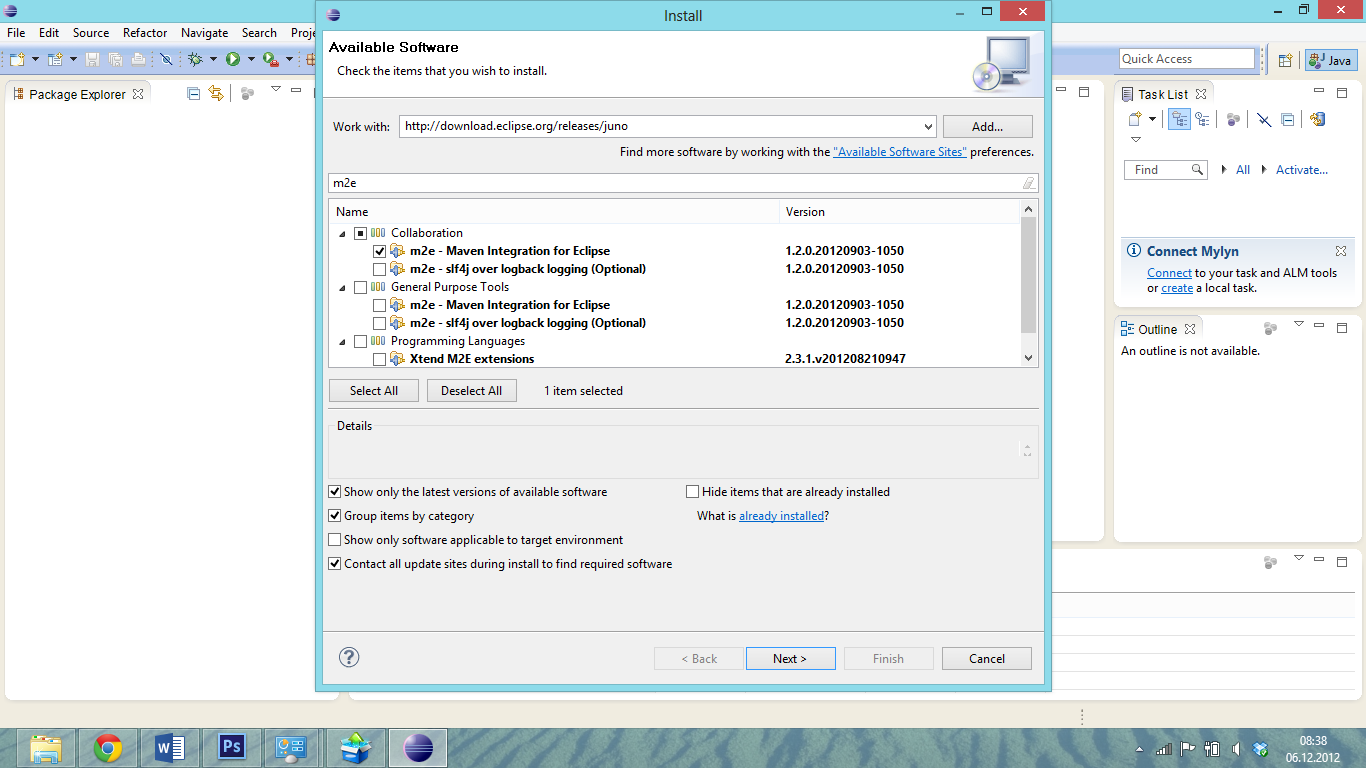
\includegraphics[width=\textwidth]{m2eplugin}
	\caption{Maven Eclipse plugin installation}
	\label{fig:m2eplugin}
\end{figure}




\subsection{Git or Egit for Eclipse}
If you have installed Juno, Egit is already integrated. If not so, you can download Egit from \href{http://download.eclipse.org/egit/updates}{here}. Or you get and install Git from \href{http://git-scm.com/download/}{here}.
	


\subsection{Modelbus Team Provider for Eclipse}
The update site for the Modelbus Team Provider is \href{http://www.modelbus.org/modelbus/downloads/current/site}{here}. Select only the ModelBus Team Provider for the installation.



\subsection{Modelbus and Metrino}
Request \href{http://www.modelbus.org/modelbus/}{the Modelbus developers} for a version of Modelbus with an integrated Metrino service. Make sure that the following Jars lie in the plugin folder of Modelbus:
\begin{itemize}
	\item de.fraunhofer.fokus.metrino.ruleEvaluator
	\item de.fraunhofer.fokus.metrino.measure
\end{itemize}
Extract Modelbus to any location in your file system. Now you have to setup the configuartaion file of Modelbus. Open the "modelbus.config" in the "serverConfiguration" folder of your modelbus installation. Set the "repositoryLocation" to "http://localhost:8080/modelbusrepository" and the "svnRepositoryLocation" to "repository":
\begingroup
    \fontsize{10pt}{12pt}\selectfont
    \begin{verbatim}  
<?xml version="1.0" encoding="UTF-8"?>
<config:ConfigModel xmi:version="2.0" xmlns:xmi="http://www.omg.org/XMI" 
  xmlns:config="http://www.modelbus.org/system/model/config.ecore">
  <locations name="repositoryLocation" location="http://localhost:8080/modelbusrepository"/>
<!-- <locations name="secureRepositoryLocation" location="https://0.0.0.0:8181/modelbusrepository">
    <properties name="SSLTrustStore" value="SSL/cacerts.jks"/>
    <properties name="SSLTrustStorePassword" value="password"/>
    <properties name="SSLKeyStore" value="SSL/modelbus.keystore"/>
    <properties name="SSLKeyStorePassword" value="password"/>
    <properties name="SSLAlgorithm" value="RSA"/>
    <properties name="SSLPassword" value="password"/>
  </locations> //-->
  <locations name="notificationLocation" location="tcp://localhost:61616"/>
  <locations name="svnRepositoryLocation" location="repository"/>
</config:ConfigModel>
    \end{verbatim}  
\endgroup
Then you will have to set some environment variables. Set
\begin{itemize}
	\item MODELBUS\_ROOT to the folder of your Modelbus installation
	\item MODELBUS\_NOTIFICATION\_LOCATION  to "tcp://localhost:61616" like in the config file
	\item MODELBUS\_REPOSITORY\_LOCATION to \\
	"http://localhost:8080/modelbusrepository" like in the config file
\end{itemize}



\section{Usage Manual}

The typical workflow for plugin development is:
\begin{enumerate}
	\item start Modelbus
	\item open the plugin project with Eclipse 
	\item make some changes to the code
	\item build the project with the Maven goal "install"
	\item deploy Sonar including out plugin via Maven
	\item analyse the project with the goal "sonar:sonar" to test the plugin on your installed Modelbus repository
\end{enumerate}

The typical workflow for an user of our plugin is:
\begin{enumerate}
	\item start ModelBus
	\item start Sonar with our plugin via Maven
	\item check in models into the Modelbus repository
	\item analyse a Maven project with the goal "sonar:sonar" (this will also analyse your installed Modelbus repository)
\end{enumerate}

The single steps are described below in detail.



\subsection{Download the source of our Sonar-Modelbus-Plugin}
Download the following copy of our repository:

\url{https://github.com/arsenij-solovjev/sonar-modelbus-plugin/archive/master.zip}

Extract the archive and if you like copy the folder sonar-modelbus-plugin-master into a special folder. It is just important that you don't copy this folder in your Eclipse workspace.



\subsection{Start Modelbus}
Under Windows start the "startModelBusServer.exe" of your Modelbus installation.

Under Linux run the "startup.sh" as root user. Make sure that the "startup.sh" and the "bin/service" files are executable.

If Modelbus is up, you can visit the Modelbus manager under \url{http://localhost:8080/modelbus?startup=manager}: You can login with the username "Admin" and the password "ModelBus". Here you can see all the checked in files and models. When uploading a new file, press the refresh button to see the changes.

\begin{figure}
	\centering
		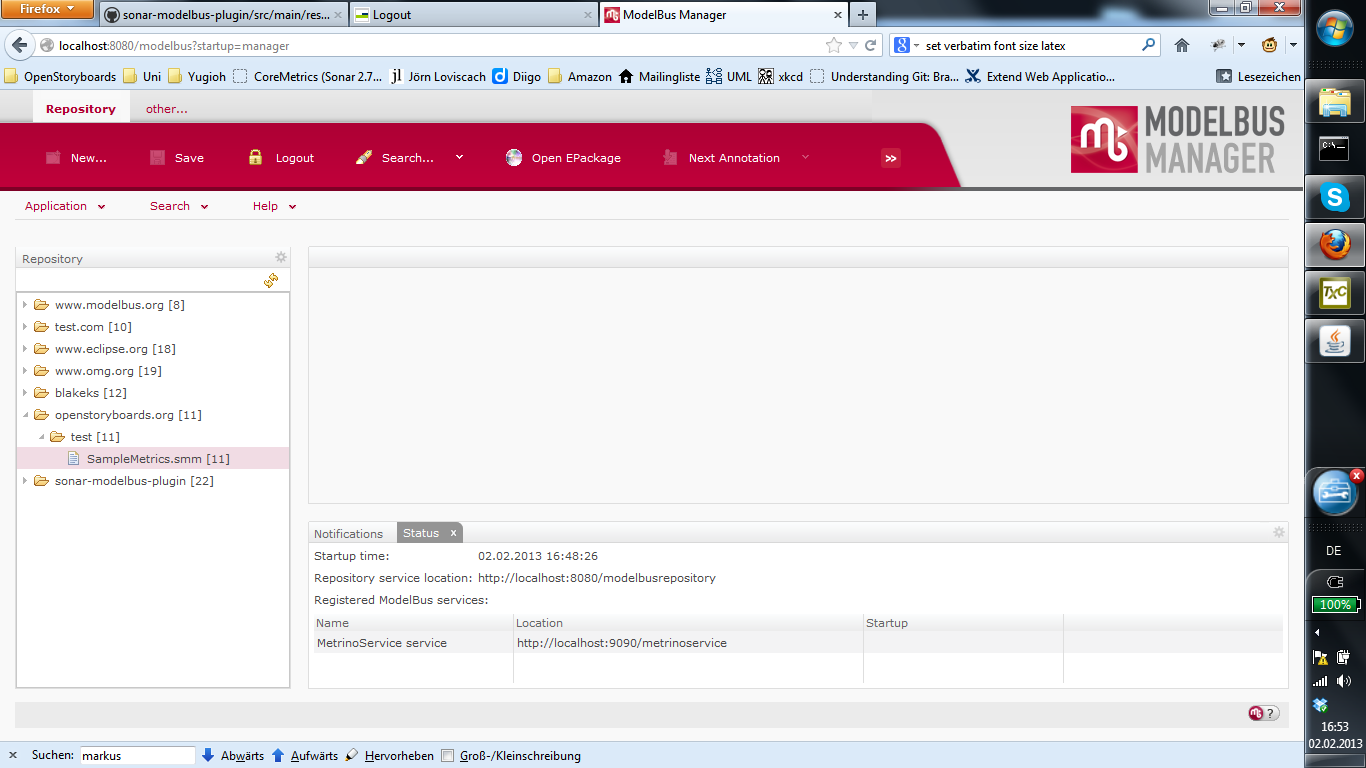
\includegraphics[width=\textwidth]{modelbusmanager}
	\caption{The Modelbus manager}
	\label{fig:modelbusmanager}
\end{figure}


\subsection{Uploading models}
We created a tool for checking in and out files from/to the ModelBus repository. It can be simply called via "make". First compile the tool: Go to the "modelbusclient/sonar-modelbus-client" folder and run:
\begin{verbatim}
make install
\end{verbatim}
This will compile and package the tool. Next, checkin some models to the Modelbus repository using:
\begin{verbatim}
make checkin 
  URI=http://uri.de/location/in/repository/file.txt 
  FILENAME=location/to/local/file.txt
\end{verbatim}
You can find some example models in the "/src/main/resources/metrinostuff" folder of our plugin.


\subsection{Create a new Eclipse project}
Now create a new Eclipse project:

\begin{figure}
	\centering
		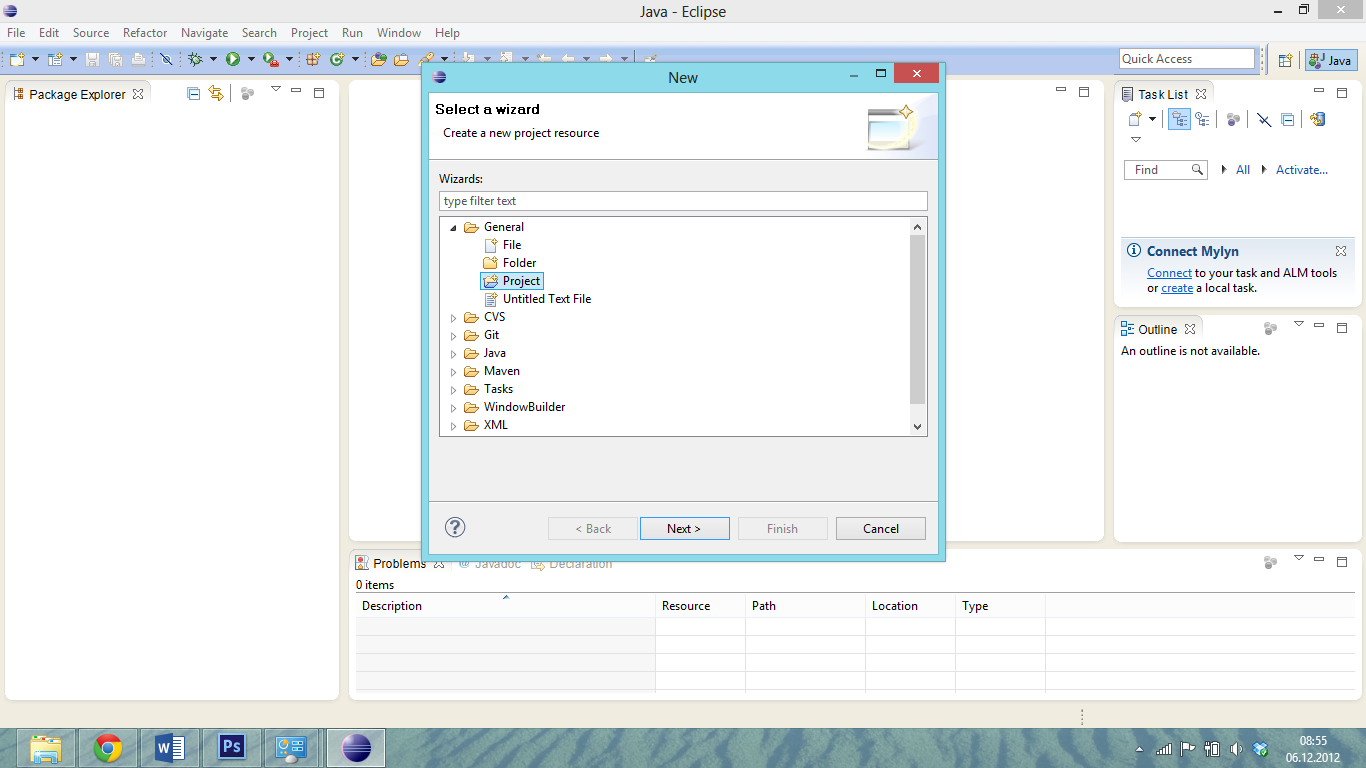
\includegraphics[width=\textwidth]{neweclipseproject}
	\caption{Creating a new Eclispe project}
	\label{fig:neweclipseproject}
\end{figure}

Unselect the "Use default location" box and select the sonar-modelbus-plugin-master folder. Don't forget to set a project name.
 
\begin{figure}
	\centering
		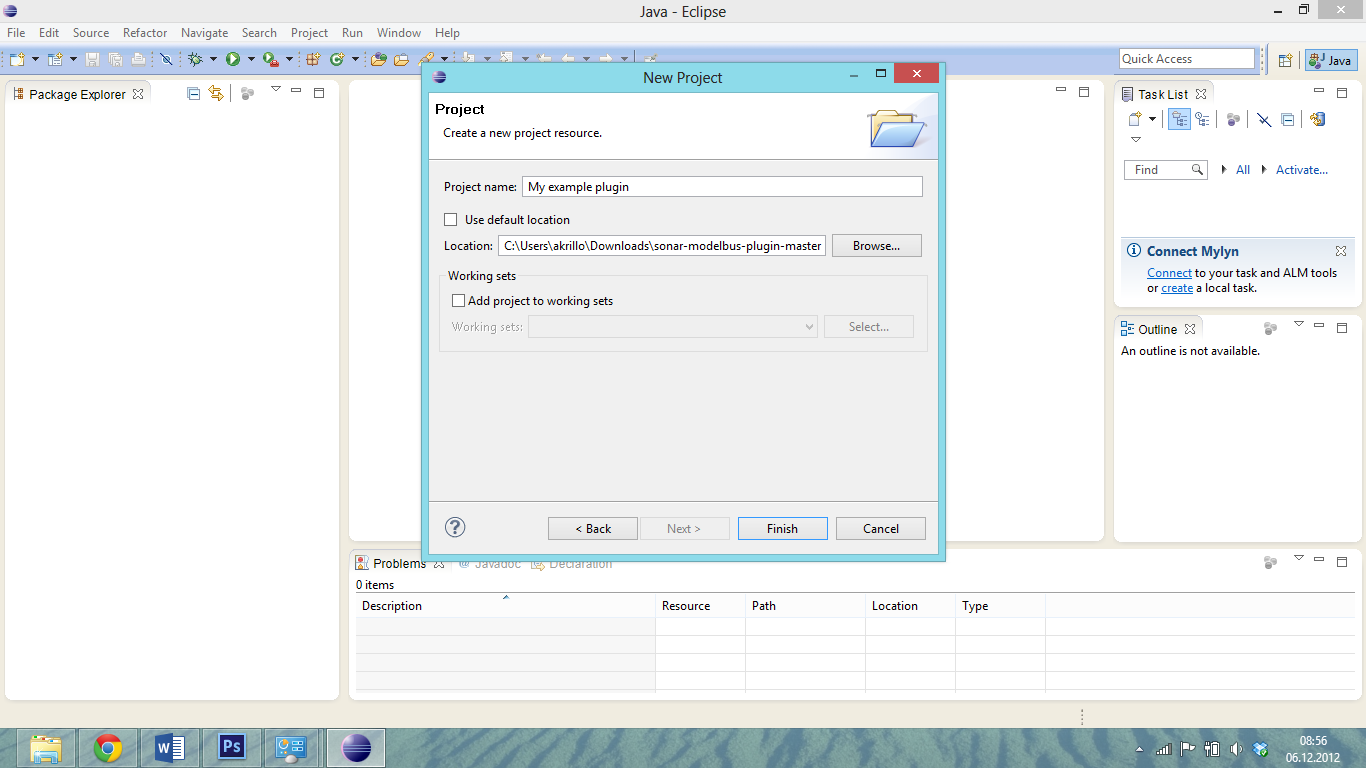
\includegraphics[width=\textwidth]{selectlocation}
	\caption{Selecting a location}
	\label{fig:selectlocation}
\end{figure}

Notice: If you finish the project creation process you may get
"Git could not detect where GIT is installed" or "check HOME directory" warning but it doesn't matter in this case.



\subsection{Convert your project to a Maven project}
Right click on your project folder and choose "Configure | Convert to Maven Project".
 
\begin{figure}
	\centering
		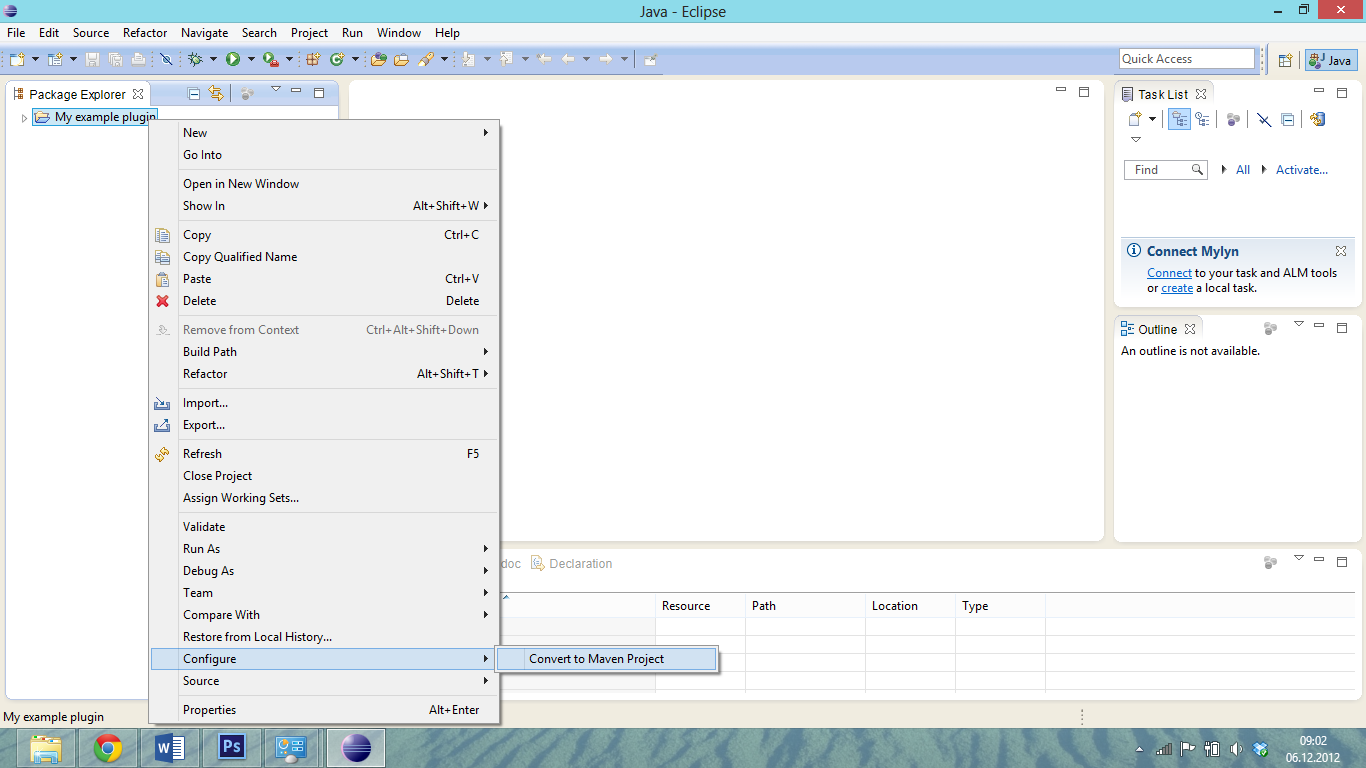
\includegraphics[width=\textwidth]{converttomavenproject}
	\caption{Converting to a Maven project}
	\label{fig:converttomavenproject}
\end{figure}

Notice: If you get any errors (this is not unusual) just ignore them. If you can't do the next step just repeat the previous one.



\subsection{Compilation}
Next: right click on your project again and select "Run as | Maven install".
\begin{figure}
	\centering
		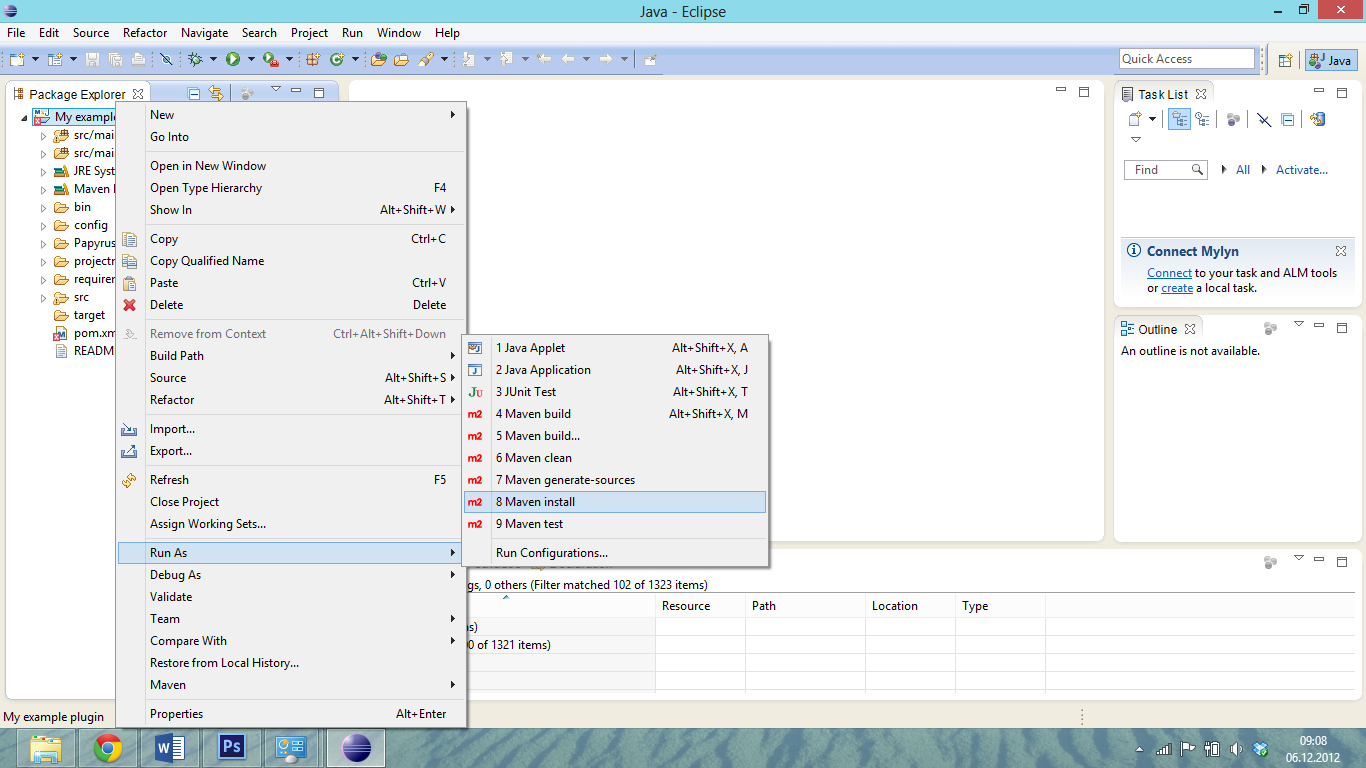
\includegraphics[width=\textwidth]{maveninstall}
	\caption{Maven install}
	\label{fig:maveninstall}
\end{figure} 
If everything works well you see a "BUILD SUCCESS" reports like this:
\begin{figure}
	\centering
		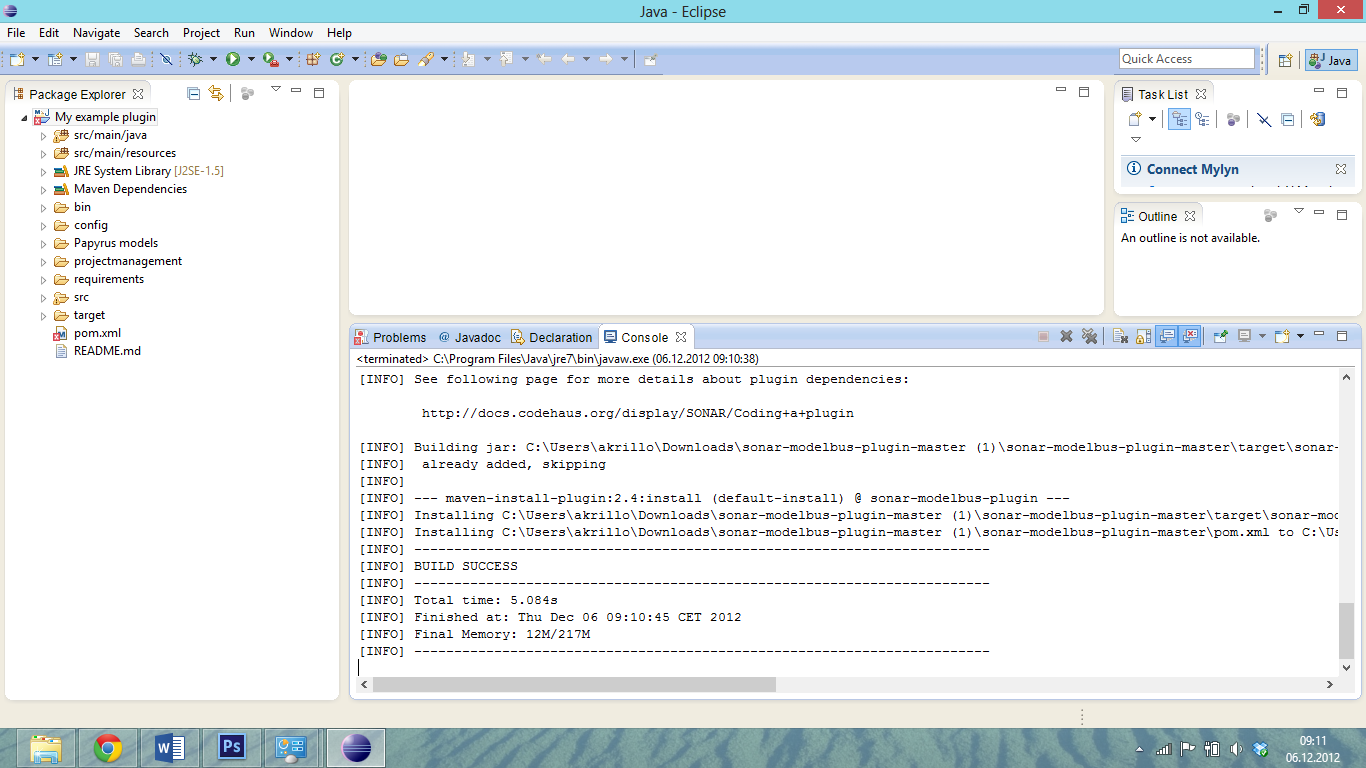
\includegraphics[width=\textwidth]{buildsuccess}
	\caption{BUILD SUCCESS}
	\label{fig:buildsuccess}
\end{figure}



\subsection{Deploy the Sonar server}
To run Sonar with our example plugin we need to run maven with an other goal. Right click on your Project and select "Run as | Maven Build". In "Goals" you must copy-paste 
\begin{verbatim}
org.codehaus.sonar:sonar-dev-maven-plugin::start-war
-Dsonar.runtimeVersion=3.3
\end{verbatim}
Then press "Run" to start the build process that will deploy a Sonar server for you. 

\begin{figure}
	\centering
		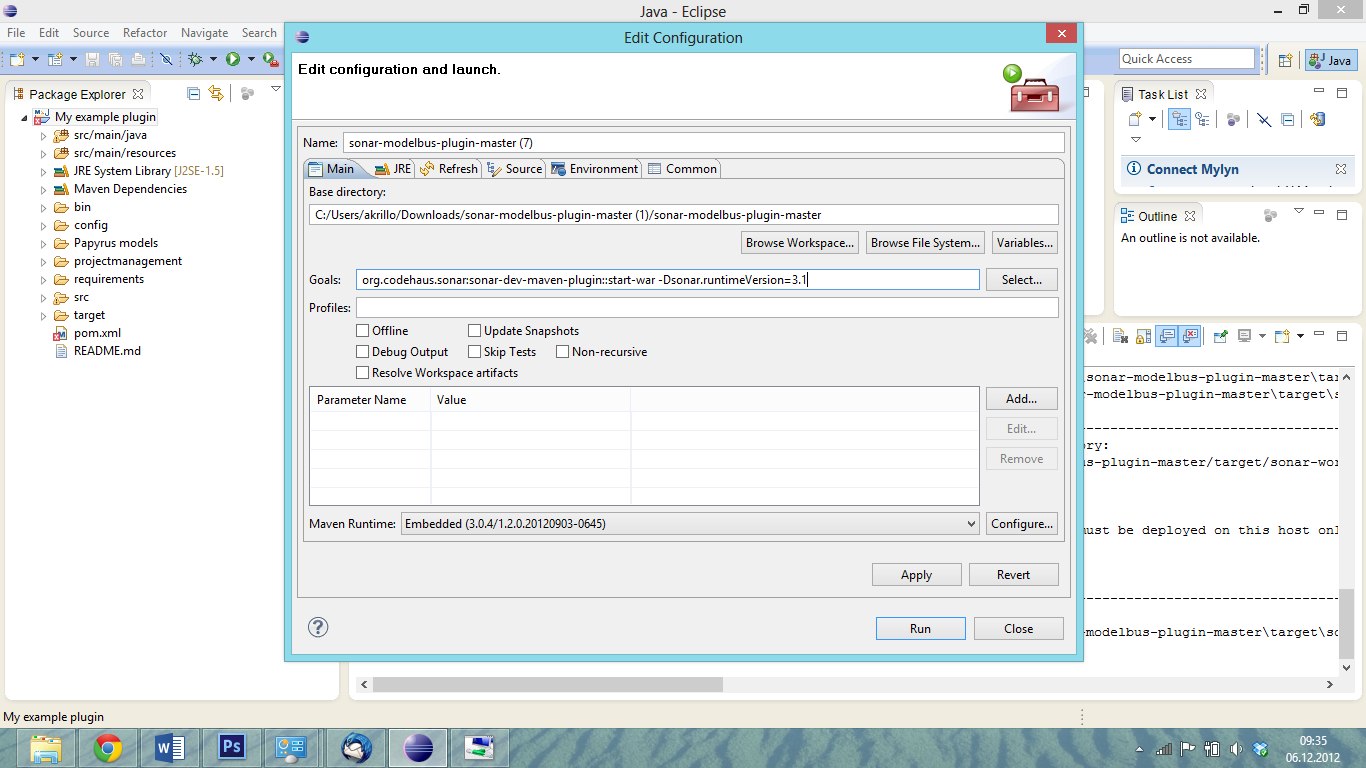
\includegraphics[width=\textwidth]{sonardeploy}
	\caption{Deploying Sonar with Maven}
	\label{fig:sonardeploy}
\end{figure}
 
Notice: this can take some minutes and if it seems to be frozen just restart the build process. If some errors occur just restart.
If everything went fine you will see following status messages:
 
\begin{figure}
	\centering
		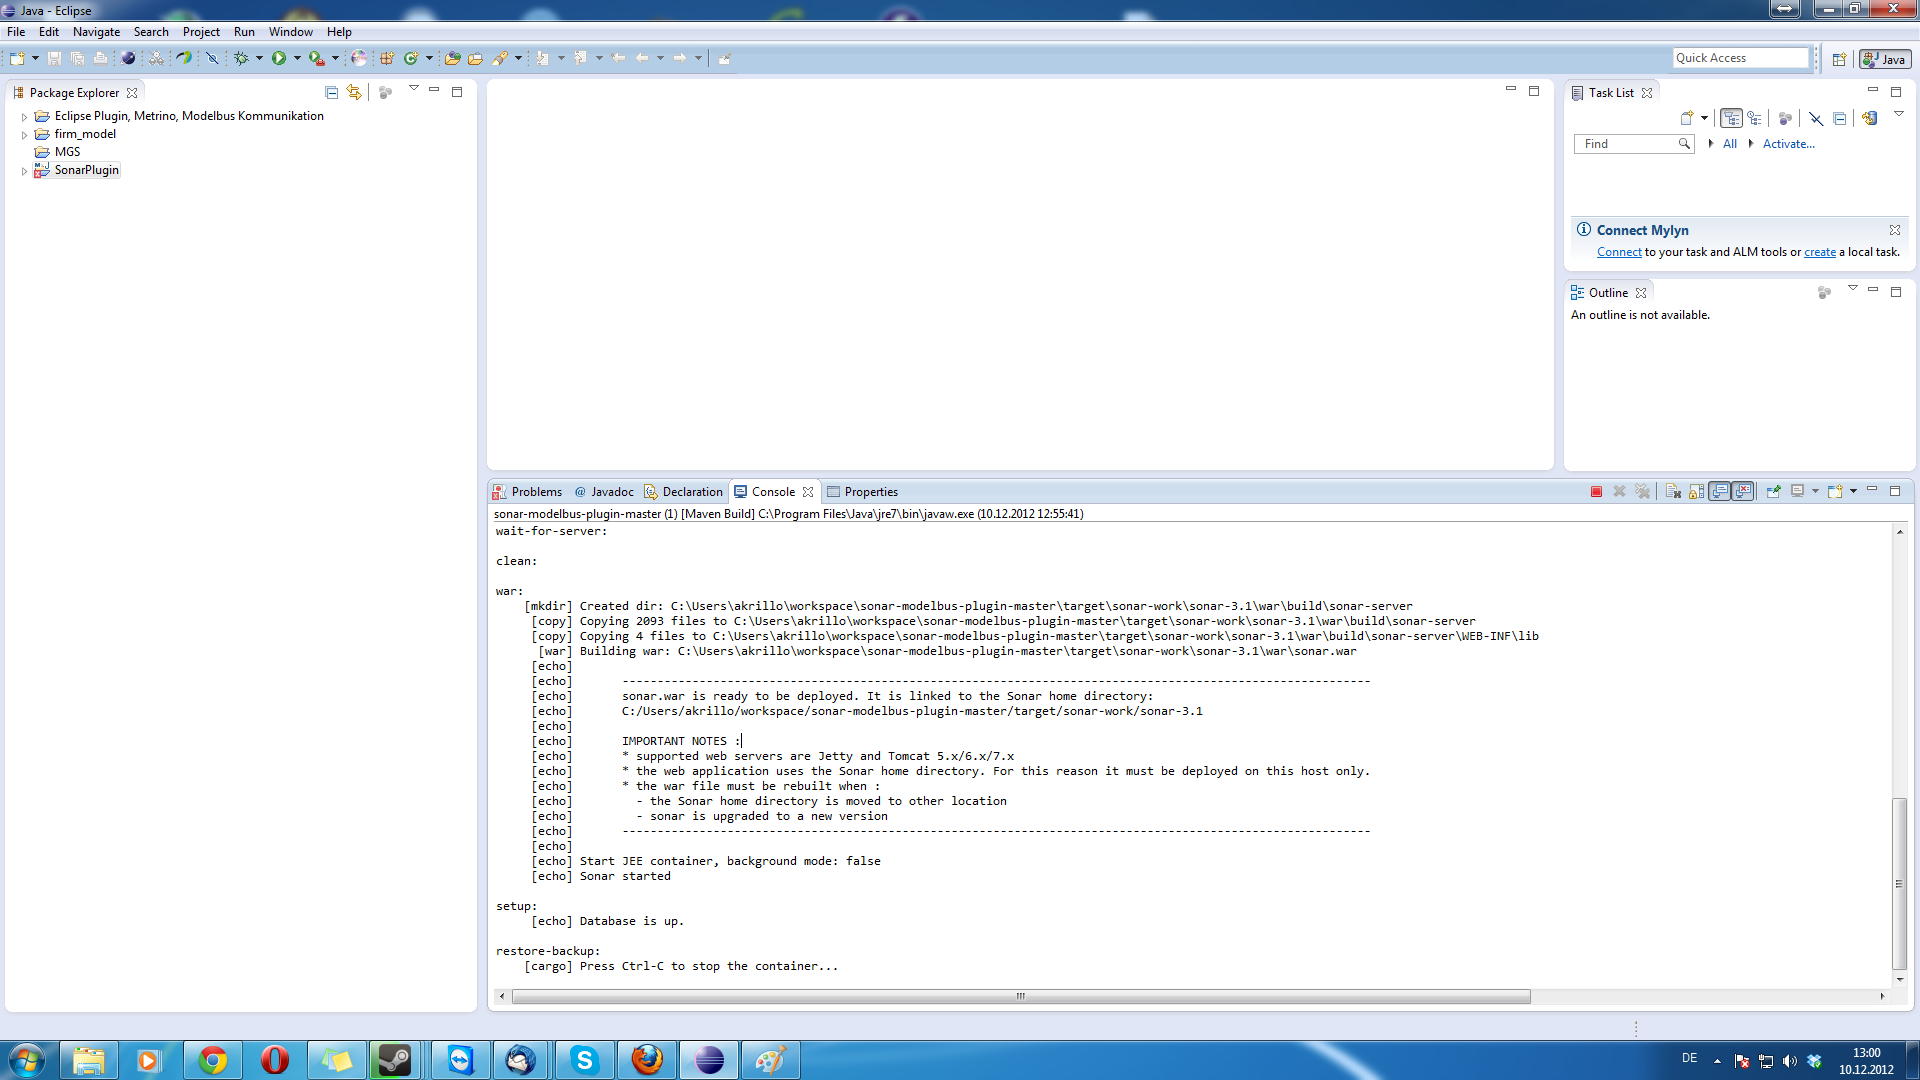
\includegraphics[width=\textwidth]{sonarready}
	\caption{Sonar is ready}
	\label{fig:sonarready}
\end{figure}

Now you can see Sonar running at "localhost:9000"  in your browser.

\begin{figure}
	\centering
		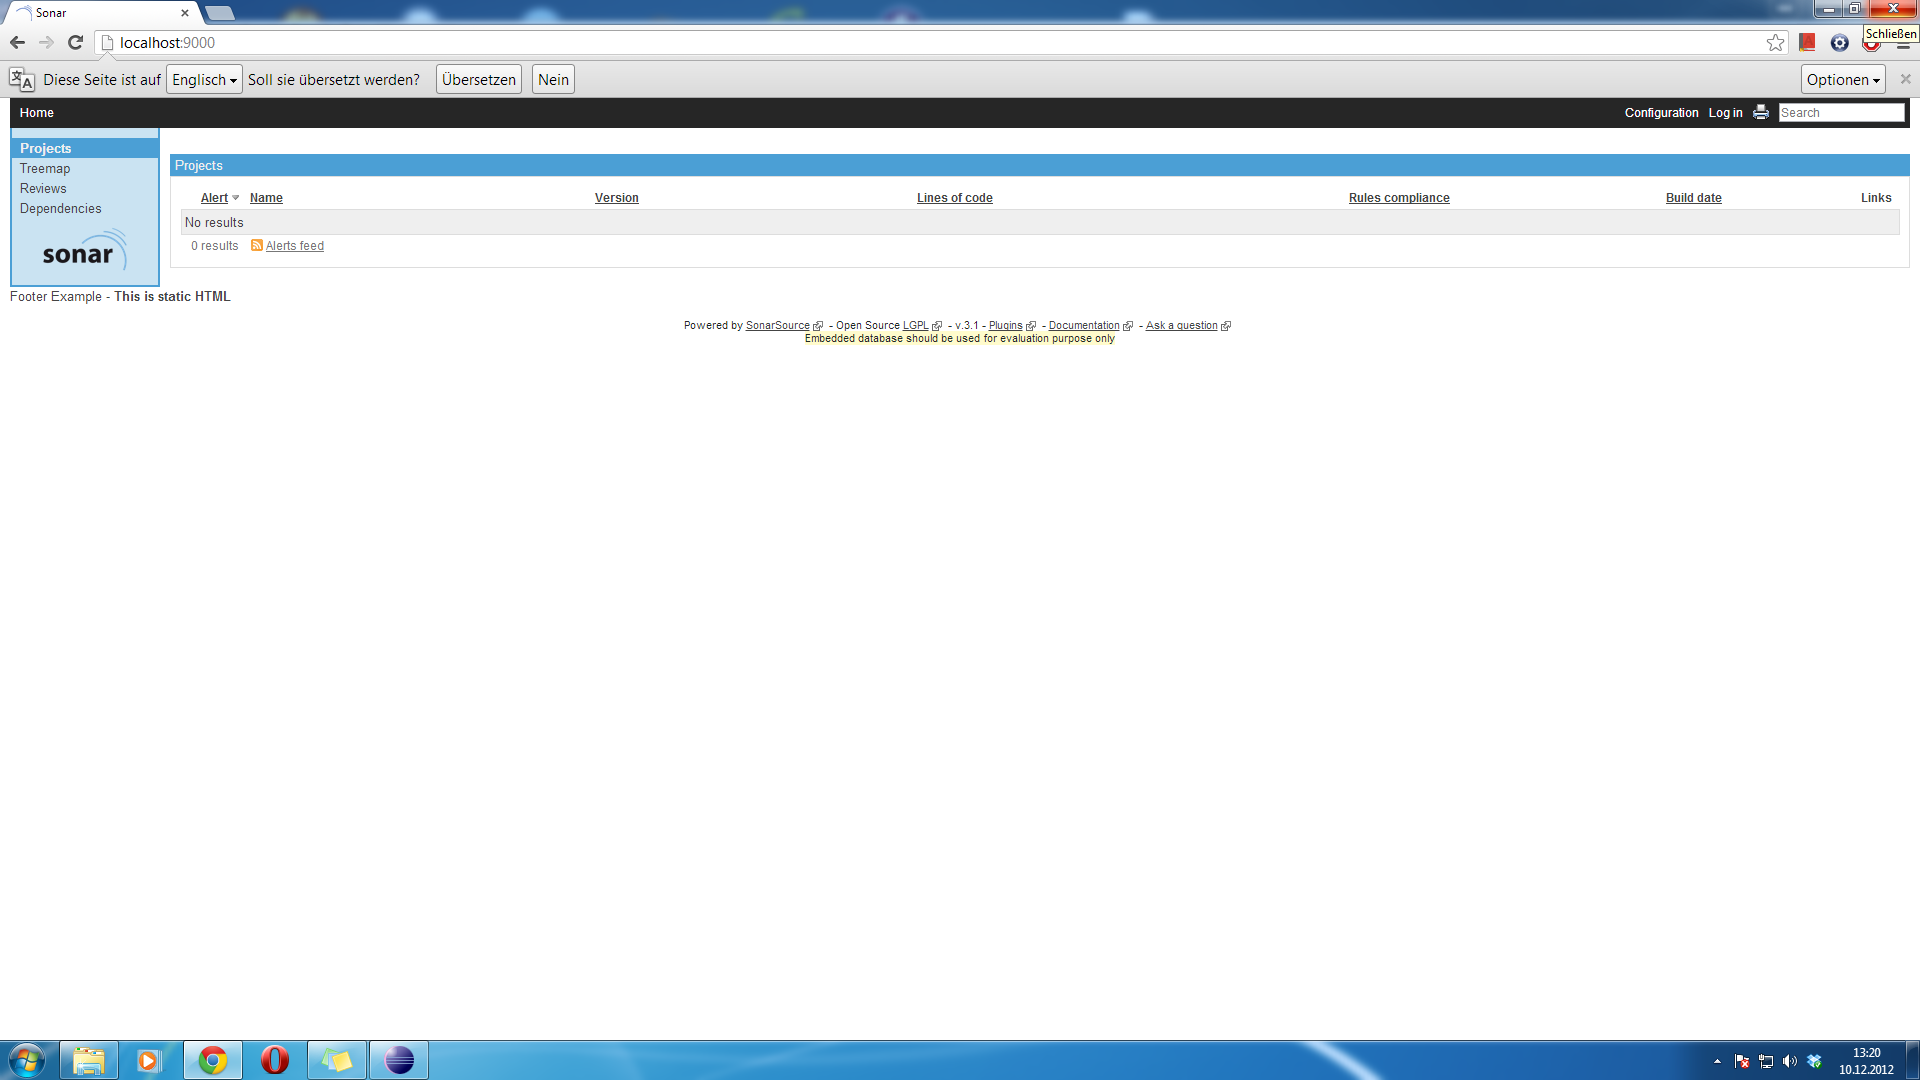
\includegraphics[width=\textwidth]{sonarrunning}
	\caption{Sonar in the browser}
	\label{fig:sonarrunning}
\end{figure}



\subsection{Analysing with Sonar}
If you like to analyse your project with Sonar (or any other Maven project) you can start the build process with the goal "sonar:sonar". After processing you can refresh your browser at "localhost:9000" and can see the results of the analysis.

\begin{figure}
	\centering
		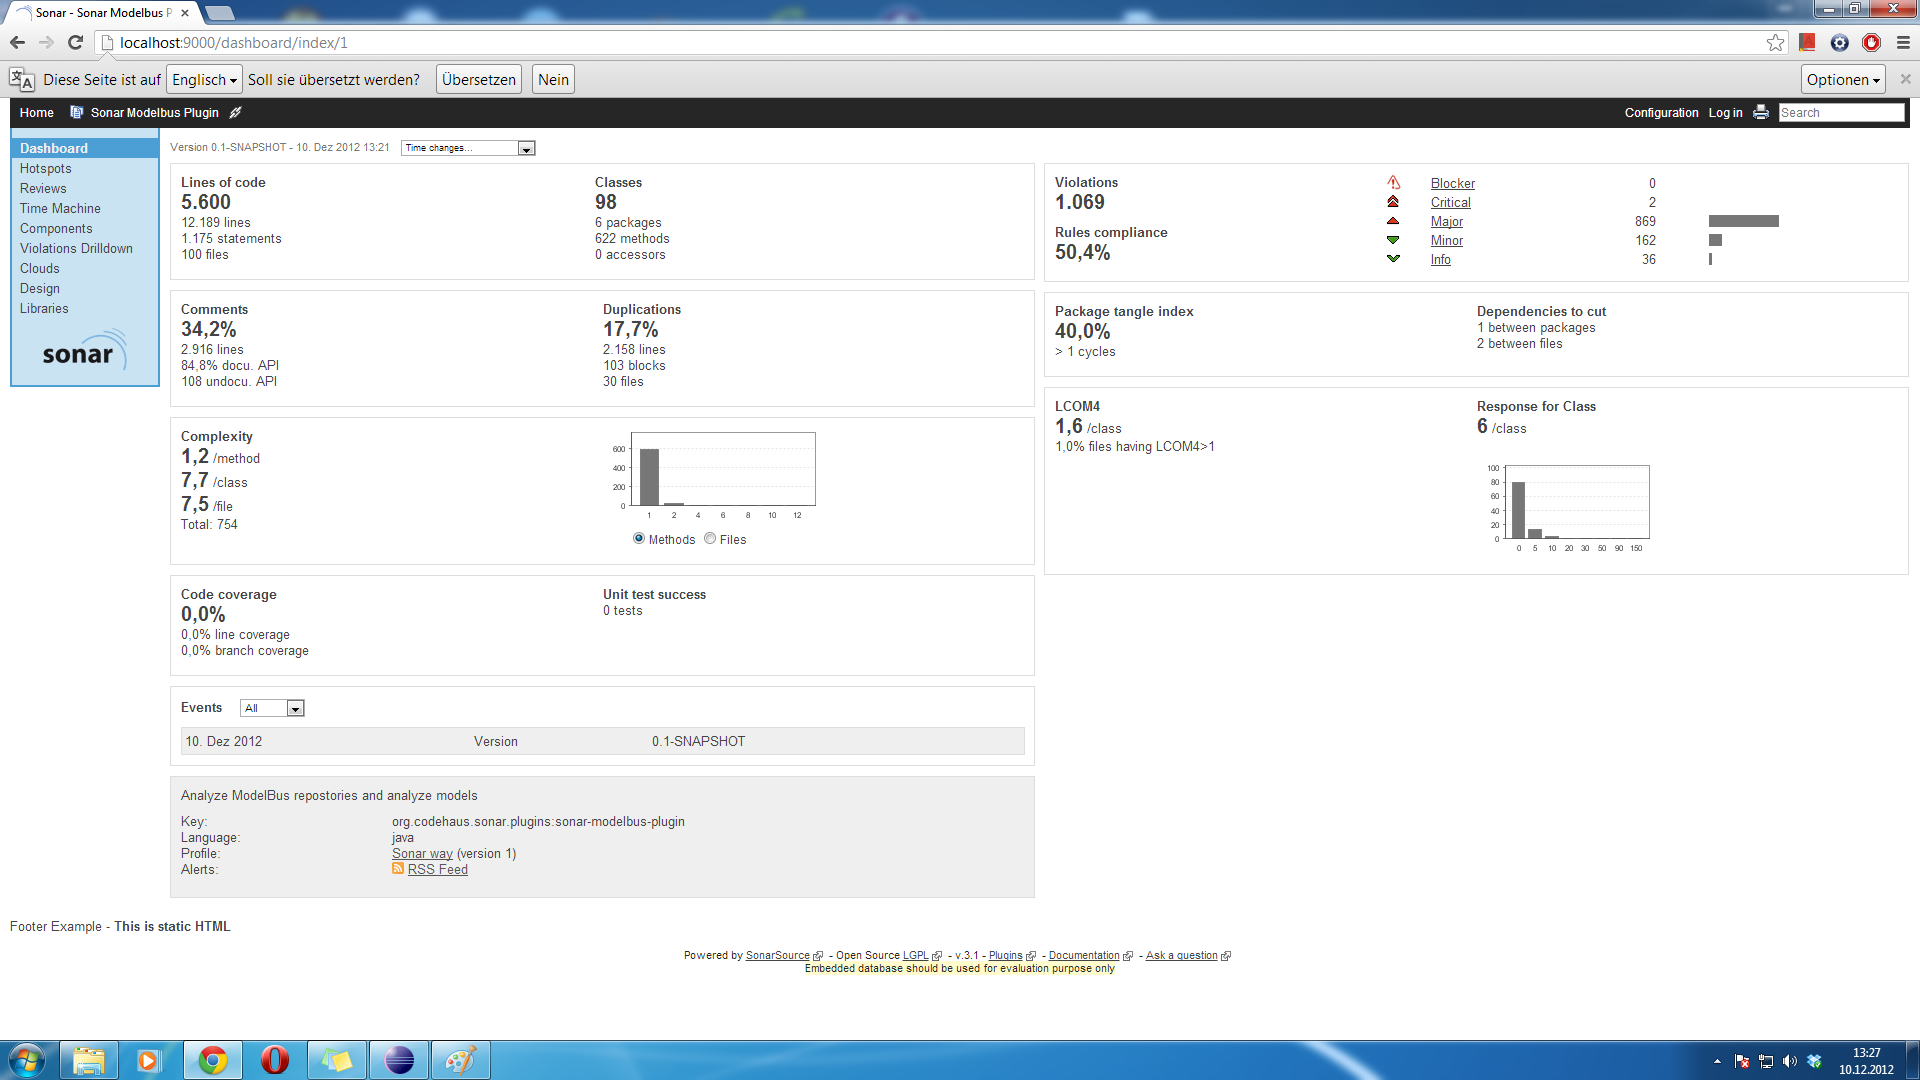
\includegraphics[width=\textwidth]{sonarinaction}
	\caption{Sonar in action}
	\label{fig:sonarinaction}
\end{figure}
\chapter{Installation and Usage} \label{sec:installation_usage}
\section{Software Requirements}
For development following software components are needed:

\begin{itemize}
	\item Java (JDK) 1.6 or 1.7
	\item Maven
  \item Eclipse (Juno)
	\item Maven Plugin for Eclipse
  \item Git or Egit for Eclipse
  \item Modelbus Team Provider for Eclipse
	\item Modelbus 1.9.7
	\item Metrino for Modelbus with following plugins
		\begin{itemize}
			\item Metrino rule evaluator plugin
			\item Metrino measure plugin
		\end{itemize}
\end{itemize}
Sonar will be downloaded and deployed via Maven at compile time.

\section{Installation Manual}
In the following sections we explain every detail. Just skip a section if you think you still have done that what the regarding section focuses. 

\subsection{Java}
We tested the software with Java 1.6 and 1.7. You can get those from \href{http://www.oracle.com/technetwork/java/javase/downloads/index.html}{here}. Select and download the current JDK to install it on your system. If Java is ready, make sure that the following system variables exist:
\begin{verbatim}
JAVA_HOME = C:\Program Files\Java\jdk1.7.0_09
(change the path to your JDK install path)
\end{verbatim}

Also you must add your JAVA\_HOME variable (add \textbackslash bin\textbackslash ) to your path variable.
\begin{verbatim}
PATH =...;%JAVA_HOME%\bin\;
\end{verbatim}

\subsection{Maven}
Download the current Maven from \href{http://maven.apache.org/download.html}{here} and follow the instructions from the README: Extract it somewhere and create following path variables:
\begin{verbatim}
M2_HOME = C:\Program Files\apache-maven-3.0.4 
(change the path to your maven folder)
M2 = %M2_HOME%\bin\
PATH =...;%M2%;
\end{verbatim}



\subsection{Eclipse}
Download Eclipse from \href{http://www.eclipse.org/juno/}{here}.
We recommend a current Eclipse version. We use Eclipse Juno (4.2) for Java developer.
Remember to select the correct version for your operating system. 



\subsection{Maven Plugin for Eclipse}
Open Eclipse and open "Help | Install New Software...". Now select or add the repository of your eclipse version. In our example we will use 

\url{http://download.eclipse.org/releases/juno}
 
Select "m2e – Maven Integration for Eclipse" and click through the progress to install the plugin. If everything works well, Eclipse will ask you for an Eclipse restart. 

\begin{figure}[h]
	\centering
		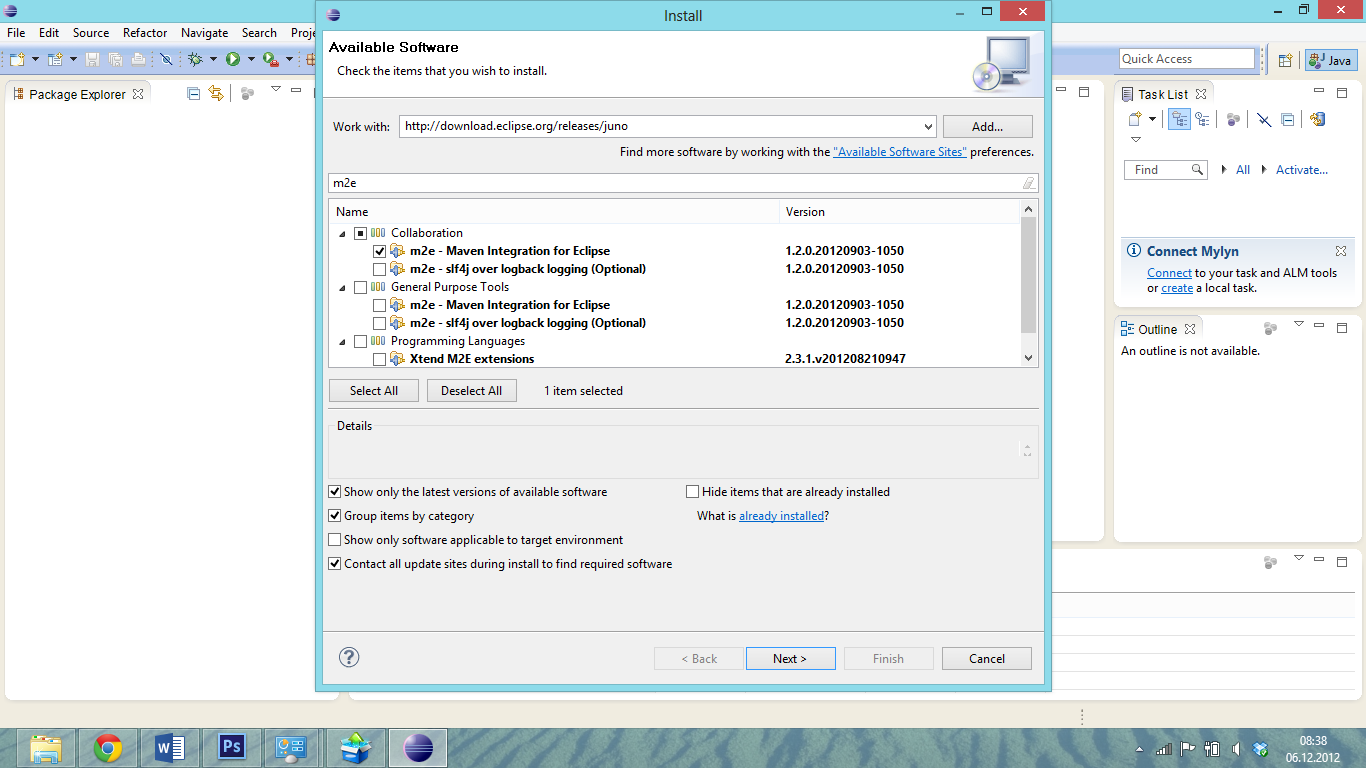
\includegraphics[width=\textwidth]{m2eplugin}
	\caption{Maven Eclipse plugin installation}
	\label{fig:m2eplugin}
\end{figure}




\subsection{Git or Egit for Eclipse}
If you have installed Juno, Egit is already integrated. If not so, you can download Egit from \href{http://download.eclipse.org/egit/updates}{here}. Or you get and install Git from \href{http://git-scm.com/download/}{here}.
	


\subsection{Modelbus Team Provider for Eclipse}
The update site for the Modelbus Team Provider is \href{http://www.modelbus.org/modelbus/downloads/current/site}{here}. Select only the ModelBus Team Provider for the installation.



\subsection{Modelbus and Metrino}
Request \href{http://www.modelbus.org/modelbus/}{the Modelbus developers} for a version of Modelbus with an integrated Metrino service. Make sure that the following Jars lie in the plugin folder of Modelbus:
\begin{itemize}
	\item de.fraunhofer.fokus.metrino.ruleEvaluator
	\item de.fraunhofer.fokus.metrino.measure
\end{itemize}
Extract Modelbus to any location in your file system. Now you have to setup the configuartaion file of Modelbus. Open the "modelbus.config" in the "serverConfiguration" folder of your modelbus installation. Set the "repositoryLocation" to "http://localhost:8080/modelbusrepository" and the "svnRepositoryLocation" to "repository":
\begingroup
    \fontsize{10pt}{12pt}\selectfont
    \begin{verbatim}  
<?xml version="1.0" encoding="UTF-8"?>
<config:ConfigModel xmi:version="2.0" xmlns:xmi="http://www.omg.org/XMI" 
  xmlns:config="http://www.modelbus.org/system/model/config.ecore">
  <locations name="repositoryLocation" location="http://localhost:8080/modelbusrepository"/>
<!-- <locations name="secureRepositoryLocation" location="https://0.0.0.0:8181/modelbusrepository">
    <properties name="SSLTrustStore" value="SSL/cacerts.jks"/>
    <properties name="SSLTrustStorePassword" value="password"/>
    <properties name="SSLKeyStore" value="SSL/modelbus.keystore"/>
    <properties name="SSLKeyStorePassword" value="password"/>
    <properties name="SSLAlgorithm" value="RSA"/>
    <properties name="SSLPassword" value="password"/>
  </locations> //-->
  <locations name="notificationLocation" location="tcp://localhost:61616"/>
  <locations name="svnRepositoryLocation" location="repository"/>
</config:ConfigModel>
    \end{verbatim}  
\endgroup
Then you will have to set some environment variables. Set
\begin{itemize}
	\item MODELBUS\_ROOT to the folder of your Modelbus installation
	\item MODELBUS\_NOTIFICATION\_LOCATION  to "tcp://localhost:61616" like in the config file
	\item MODELBUS\_REPOSITORY\_LOCATION to \\
	"http://localhost:8080/modelbusrepository" like in the config file
\end{itemize}



\section{Usage Manual}

The typical workflow for plugin development is:
\begin{enumerate}
	\item start Modelbus
	\item open the plugin project with Eclipse 
	\item make some changes to the code
	\item build the project with the Maven goal "install"
	\item deploy Sonar including out plugin via Maven
	\item analyse the project with the goal "sonar:sonar" to test the plugin on your installed Modelbus repository
\end{enumerate}

The typical workflow for an user of our plugin is:
\begin{enumerate}
	\item start ModelBus
	\item start Sonar with our plugin via Maven
	\item check in models into the Modelbus repository
	\item analyse a Maven project with the goal "sonar:sonar" (this will also analyse your installed Modelbus repository)
\end{enumerate}

The single steps are described below in detail.



\subsection{Download the source of our Sonar-Modelbus-Plugin}
Download the following copy of our repository:

\url{https://github.com/arsenij-solovjev/sonar-modelbus-plugin/archive/master.zip}

Extract the archive and if you like copy the folder sonar-modelbus-plugin-master into a special folder. It is just important that you don't copy this folder in your Eclipse workspace.



\subsection{Start Modelbus}
Under Windows start the "startModelBusServer.exe" of your Modelbus installation.

Under Linux run the "startup.sh" as root user. Make sure that the "startup.sh" and the "bin/service" files are executable.

If Modelbus is up, you can visit the Modelbus manager under \url{http://localhost:8080/modelbus?startup=manager}: You can login with the username "Admin" and the password "ModelBus". Here you can see all the checked in files and models. When uploading a new file, press the refresh button to see the changes.

\begin{figure}[h]
	\centering
		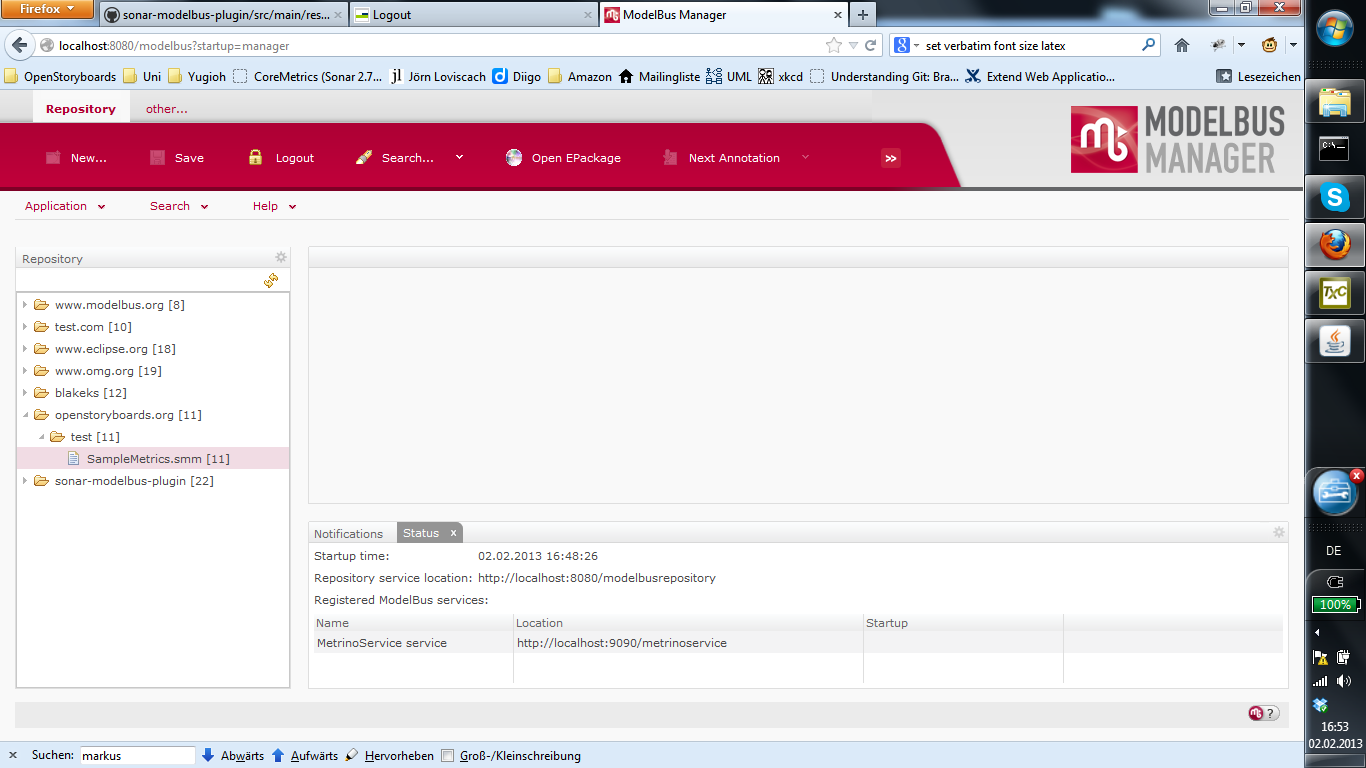
\includegraphics[width=\textwidth]{modelbusmanager}
	\caption{The Modelbus manager}
	\label{fig:modelbusmanager}
\end{figure}


\subsection{Uploading models}
We created a tool for checking in and out files from/to the ModelBus repository. It can be simply called via "make". First compile the tool: Go to the "modelbusclient/sonar-modelbus-client" folder and run:
\begin{verbatim}
make install
\end{verbatim}
This will compile and package the tool. Next, checkin some models to the Modelbus repository using:
\begin{verbatim}
make checkin 
  URI=http://uri.de/location/in/repository/file.txt 
  FILENAME=location/to/local/file.txt
\end{verbatim}
You can find some example models in the "/src/main/resources/metrinostuff" folder of our plugin.


\subsection{Create a new Eclipse project}
Now create a new Eclipse project:

\begin{figure}[h]
	\centering
		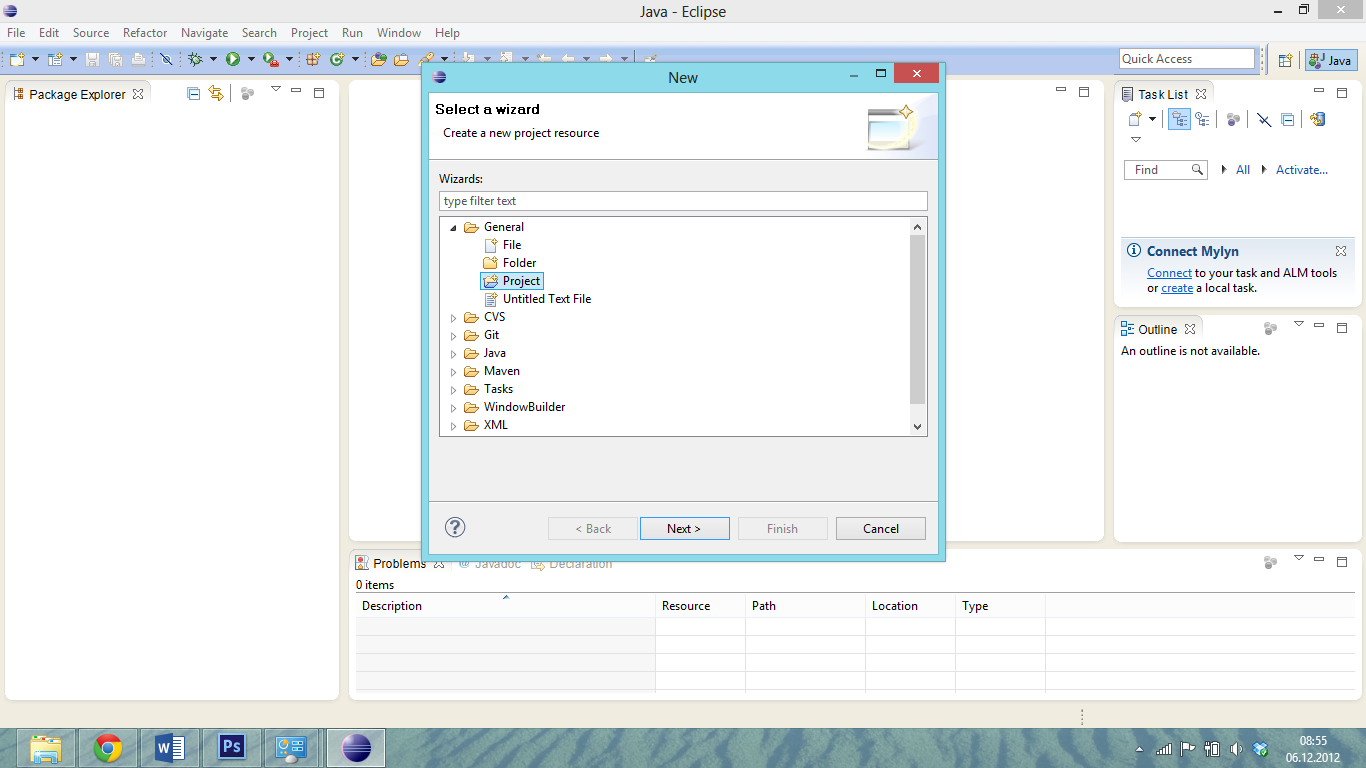
\includegraphics[width=\textwidth]{neweclipseproject}
	\caption{Creating a new Eclispe project}
	\label{fig:neweclipseproject}
\end{figure}

Unselect the "Use default location" box and select the sonar-modelbus-plugin-master folder. Don't forget to set a project name.
 
\begin{figure}[h]
	\centering
		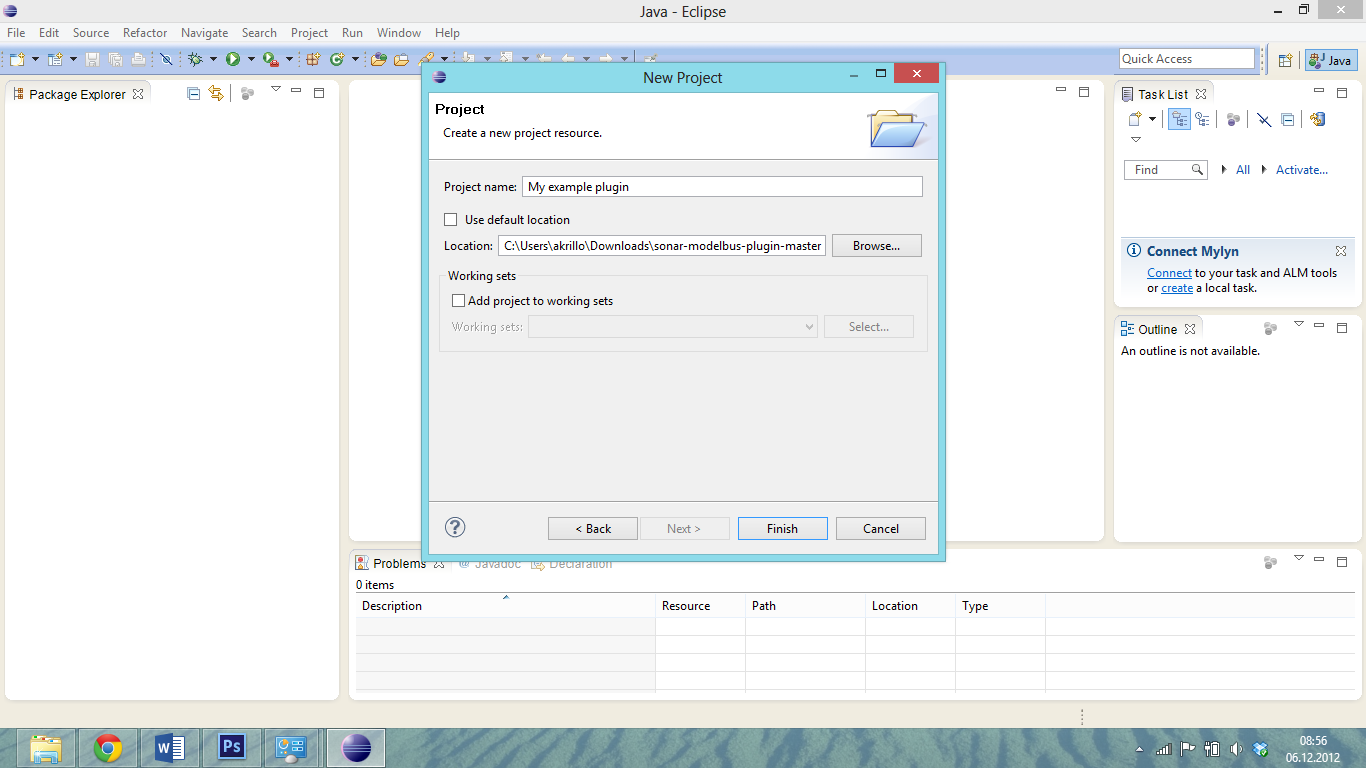
\includegraphics[width=\textwidth]{selectlocation}
	\caption{Selecting a location}
	\label{fig:selectlocation}
\end{figure}

Notice: If you finish the project creation process you may get
"Git could not detect where GIT is installed" or "check HOME directory" warning but it doesn't matter in this case.



\subsection{Convert your project to a Maven project}
Right click on your project folder and choose "Configure | Convert to Maven Project".
 
\begin{figure}[h]
	\centering
		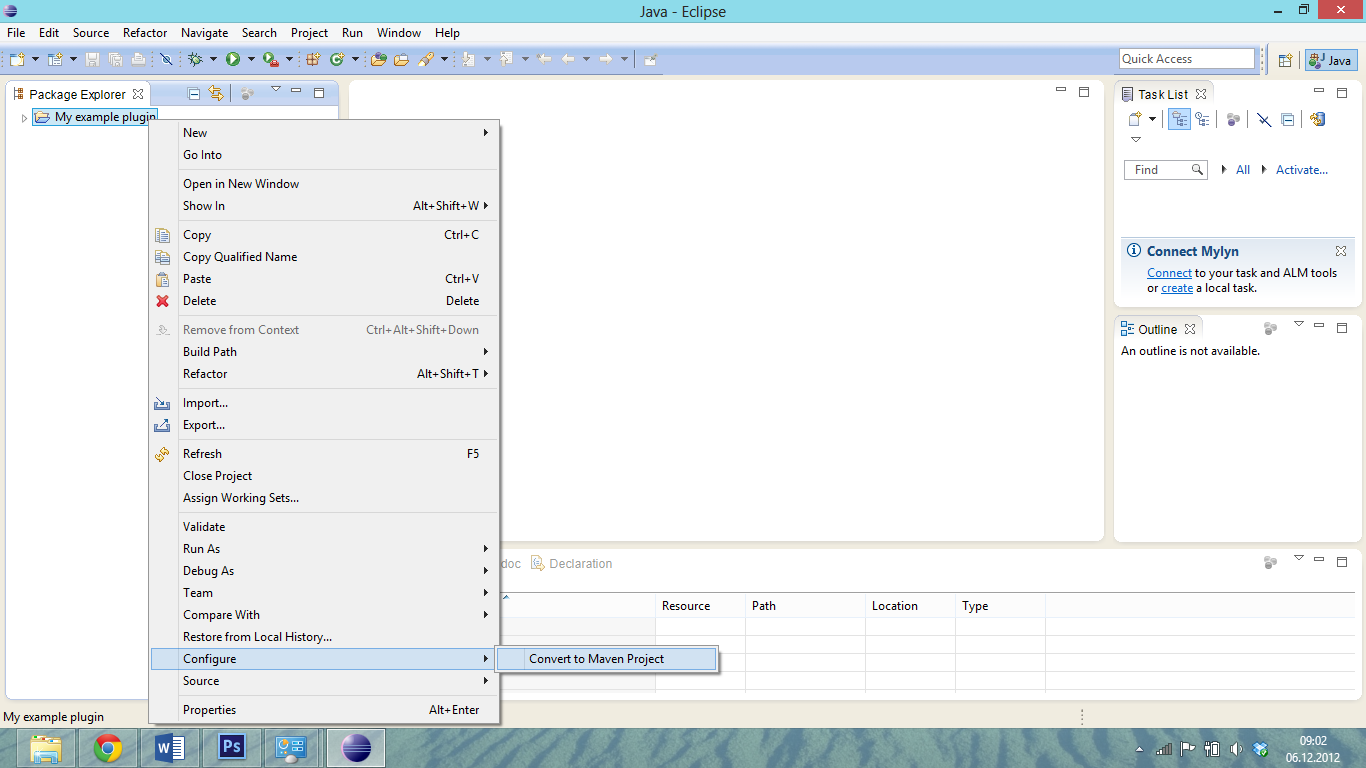
\includegraphics[width=\textwidth]{converttomavenproject}
	\caption{Converting to a Maven project}
	\label{fig:converttomavenproject}
\end{figure}

Notice: If you get any errors (this is not unusual) just ignore them. If you can't do the next step just repeat the previous one.



\subsection{Compilation}
Next: right click on your project again and select "Run as | Maven install".
\begin{figure}[h]
	\centering
		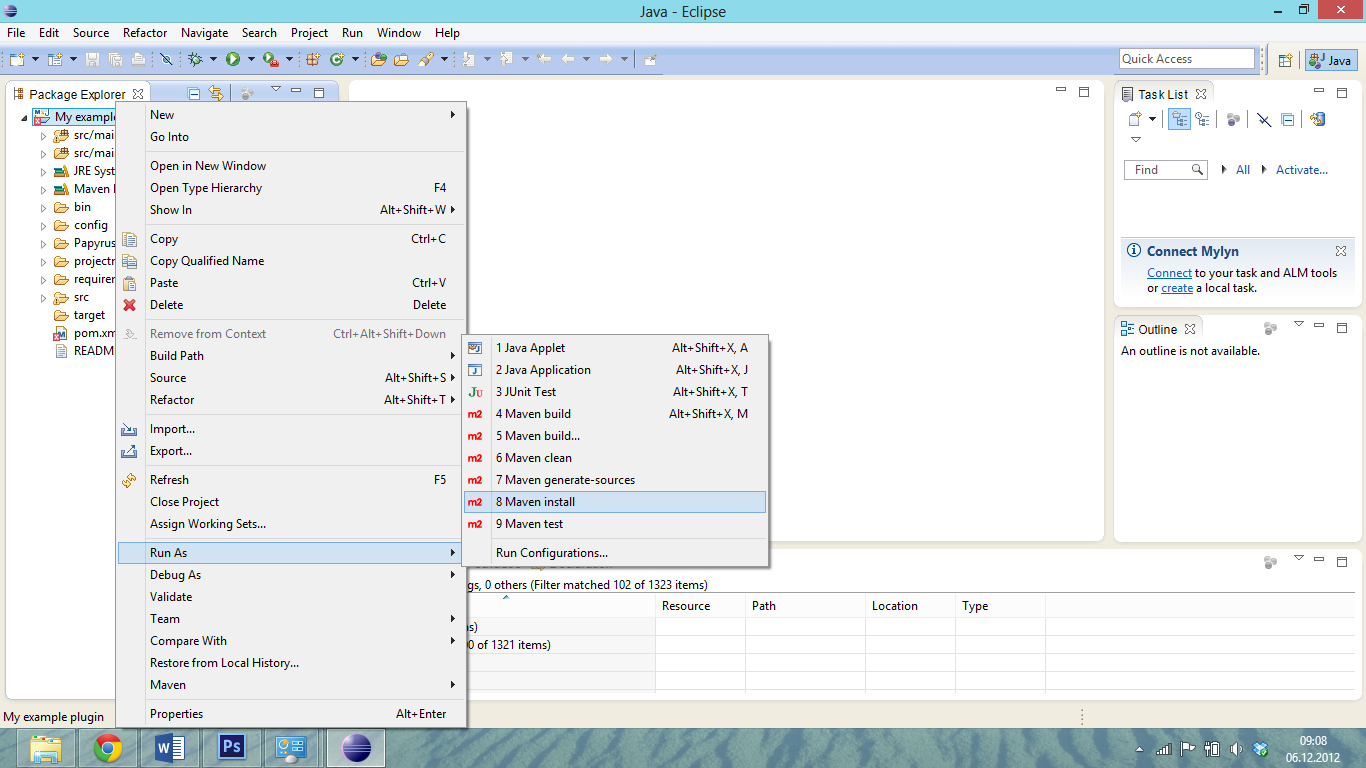
\includegraphics[width=\textwidth]{maveninstall}
	\caption{Maven install}
	\label{fig:maveninstall}
\end{figure} 
If everything works well you see a "BUILD SUCCESS" reports like this:
\begin{figure}[h]
	\centering
		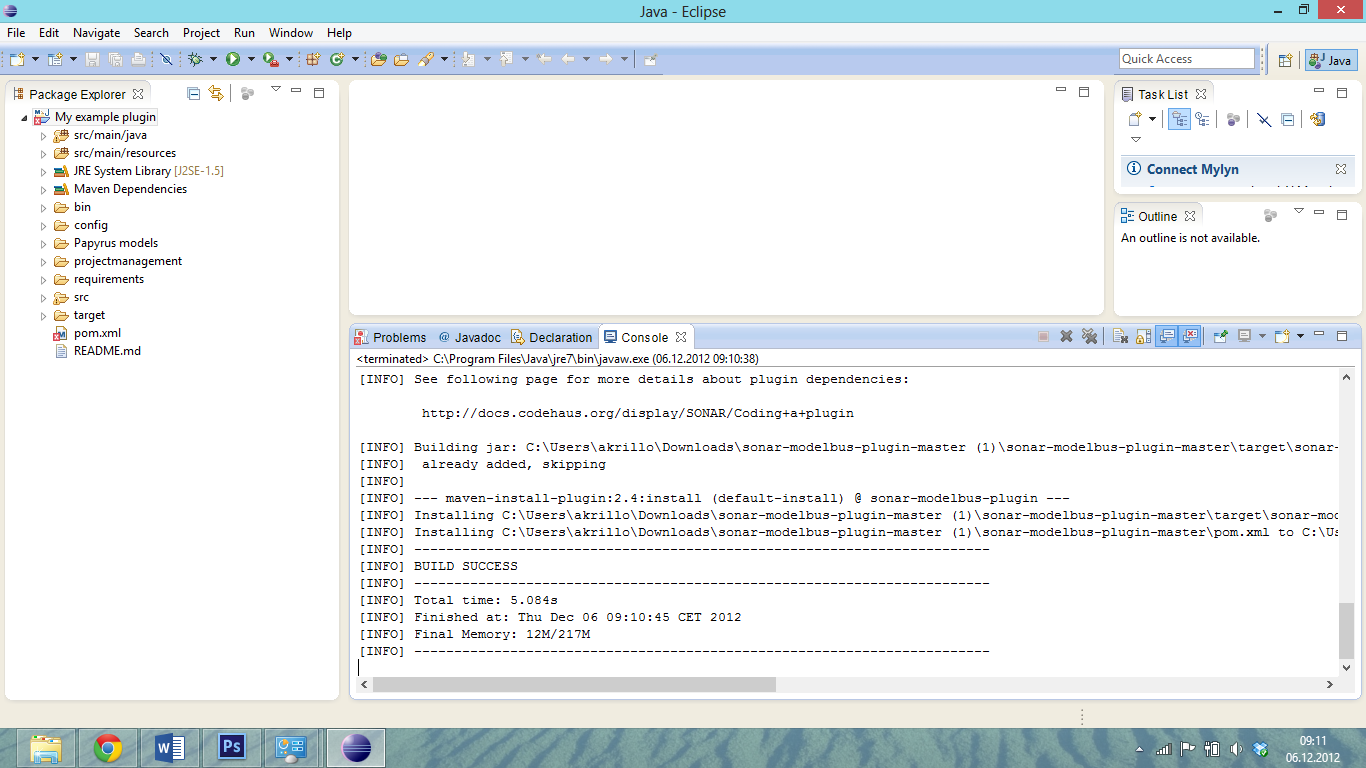
\includegraphics[width=\textwidth]{buildsuccess}
	\caption{BUILD SUCCESS}
	\label{fig:buildsuccess}
\end{figure}



\subsection{Deploy the Sonar server}
To run Sonar with our example plugin we need to run maven with an other goal. Right click on your Project and select "Run as | Maven Build". In "Goals" you must copy-paste 
\begin{verbatim}
org.codehaus.sonar:sonar-dev-maven-plugin::start-war
-Dsonar.runtimeVersion=3.3
\end{verbatim}
Then press "Run" to start the build process that will deploy a Sonar server for you. 

\begin{figure}[h]
	\centering
		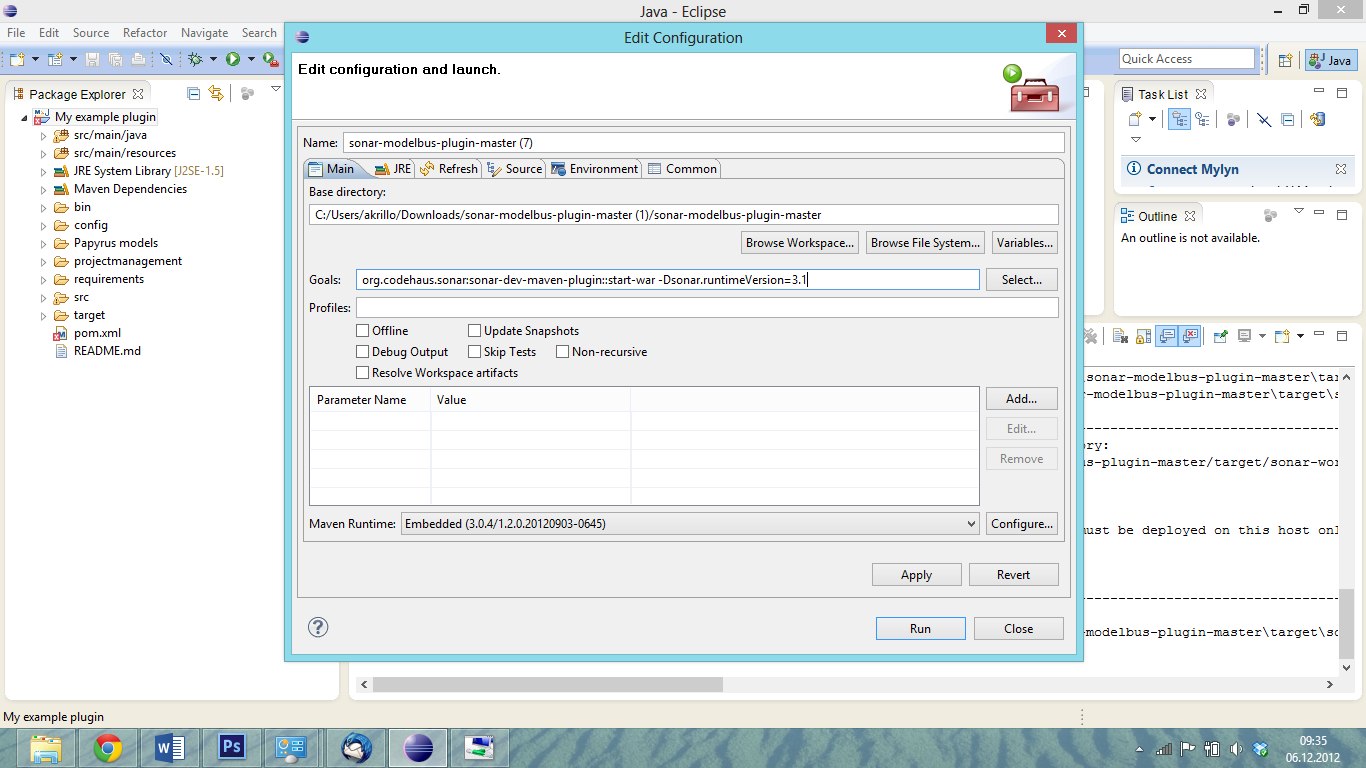
\includegraphics[width=\textwidth]{sonardeploy}
	\caption{Deploying Sonar with Maven}
	\label{fig:sonardeploy}
\end{figure}
 
Notice: this can take some minutes and if it seems to be frozen just restart the build process. If some errors occur just restart.
If everything went fine you will see following status messages:
 
\begin{figure}[h]
	\centering
		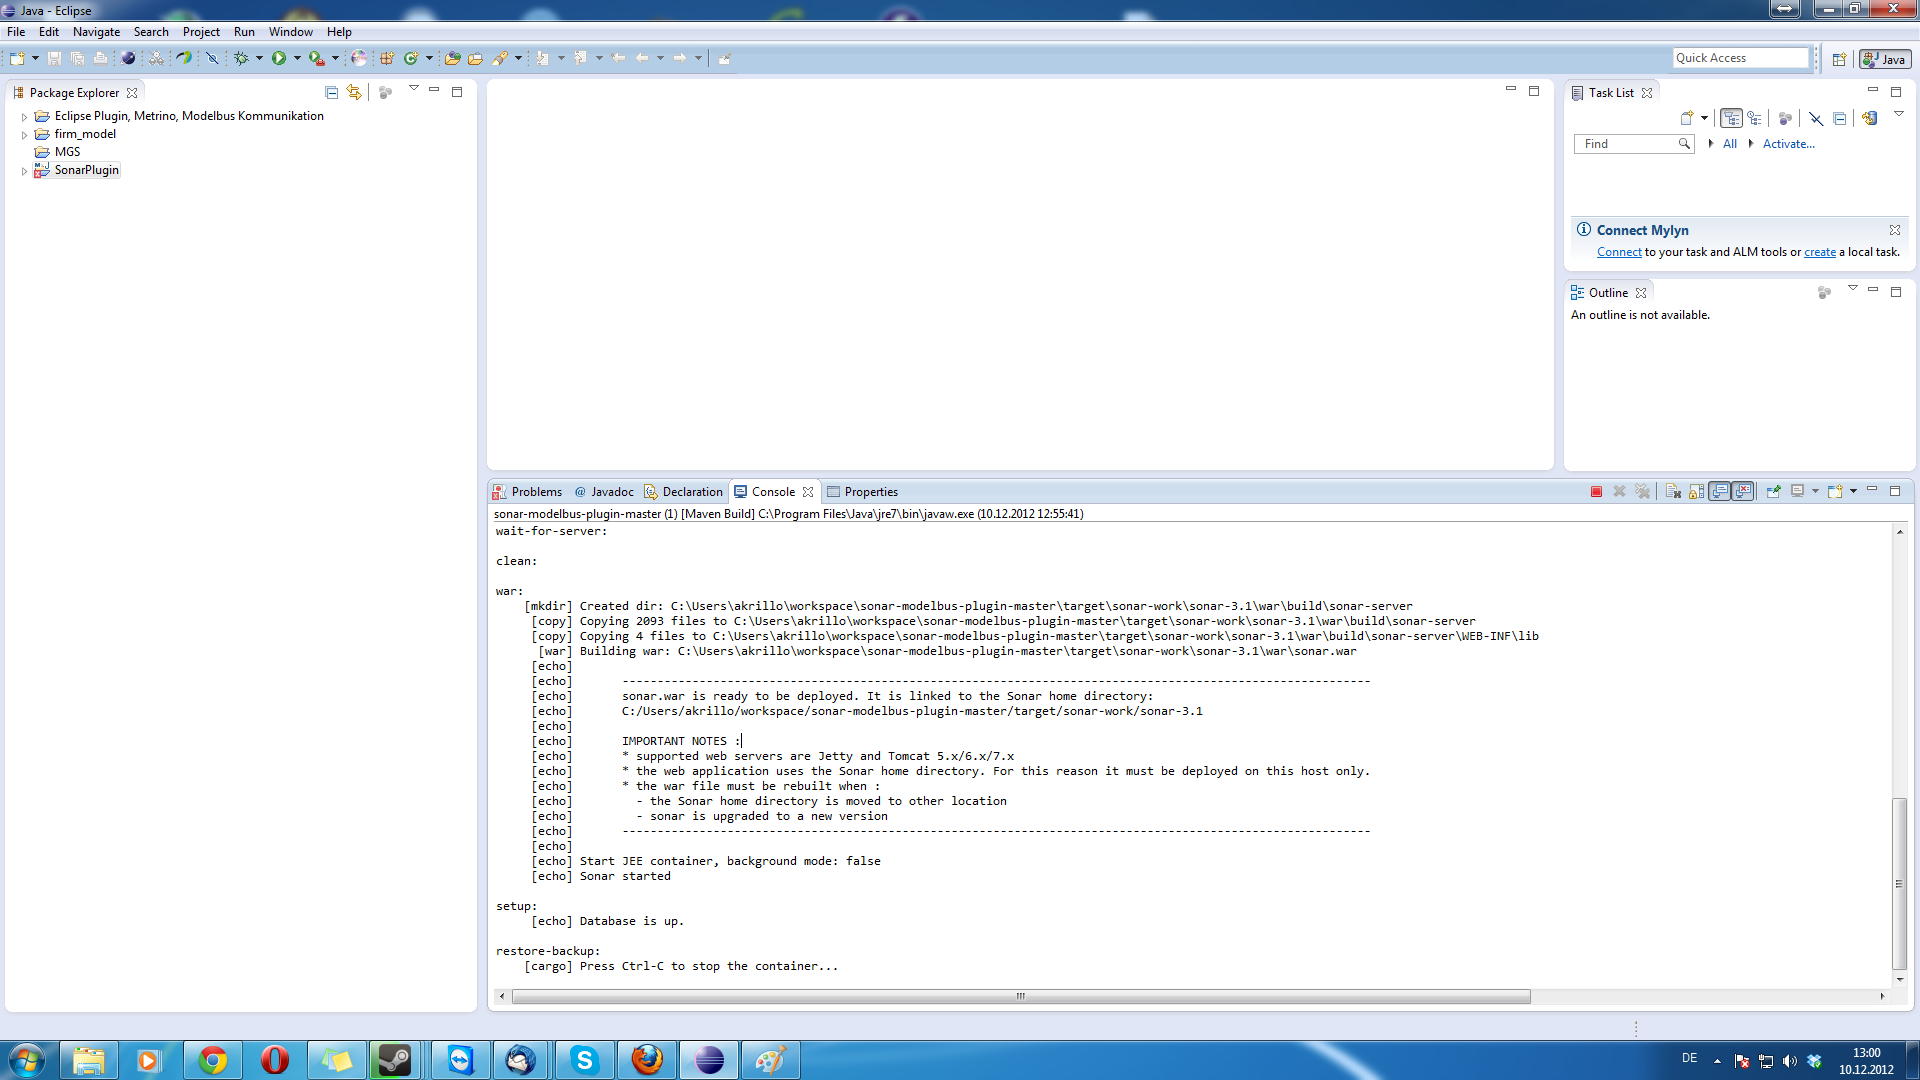
\includegraphics[width=\textwidth]{sonarready}
	\caption{Sonar is ready}
	\label{fig:sonarready}
\end{figure}

Now you can see Sonar running at "localhost:9000"  in your browser.

\begin{figure}[h]
	\centering
		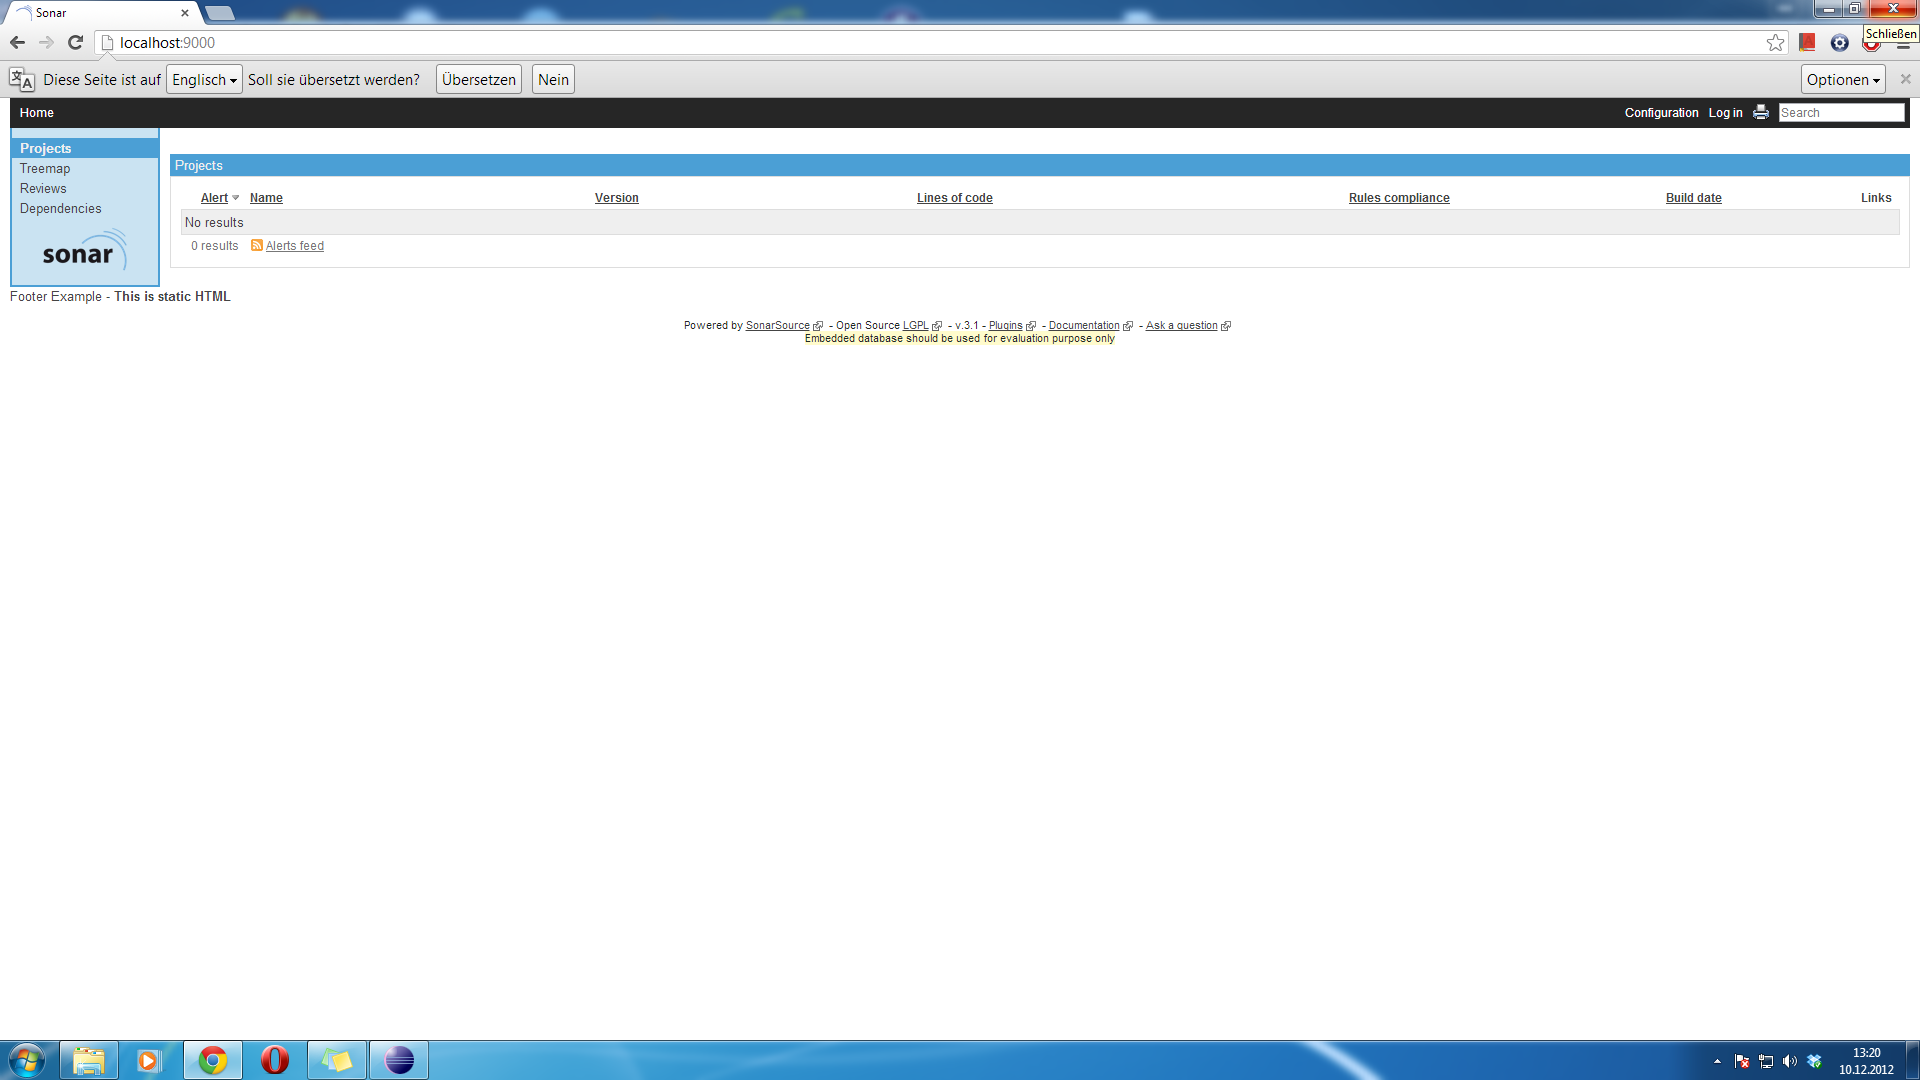
\includegraphics[width=\textwidth]{sonarrunning}
	\caption{Sonar in the browser}
	\label{fig:sonarrunning}
\end{figure}



\subsection{Analysing with Sonar}
If you like to analyse your project with Sonar (or any other Maven project) you can start the build process with the goal "sonar:sonar". After processing you can refresh your browser at "localhost:9000" and can see the results of the analysis.

\begin{figure}[h]
	\centering
		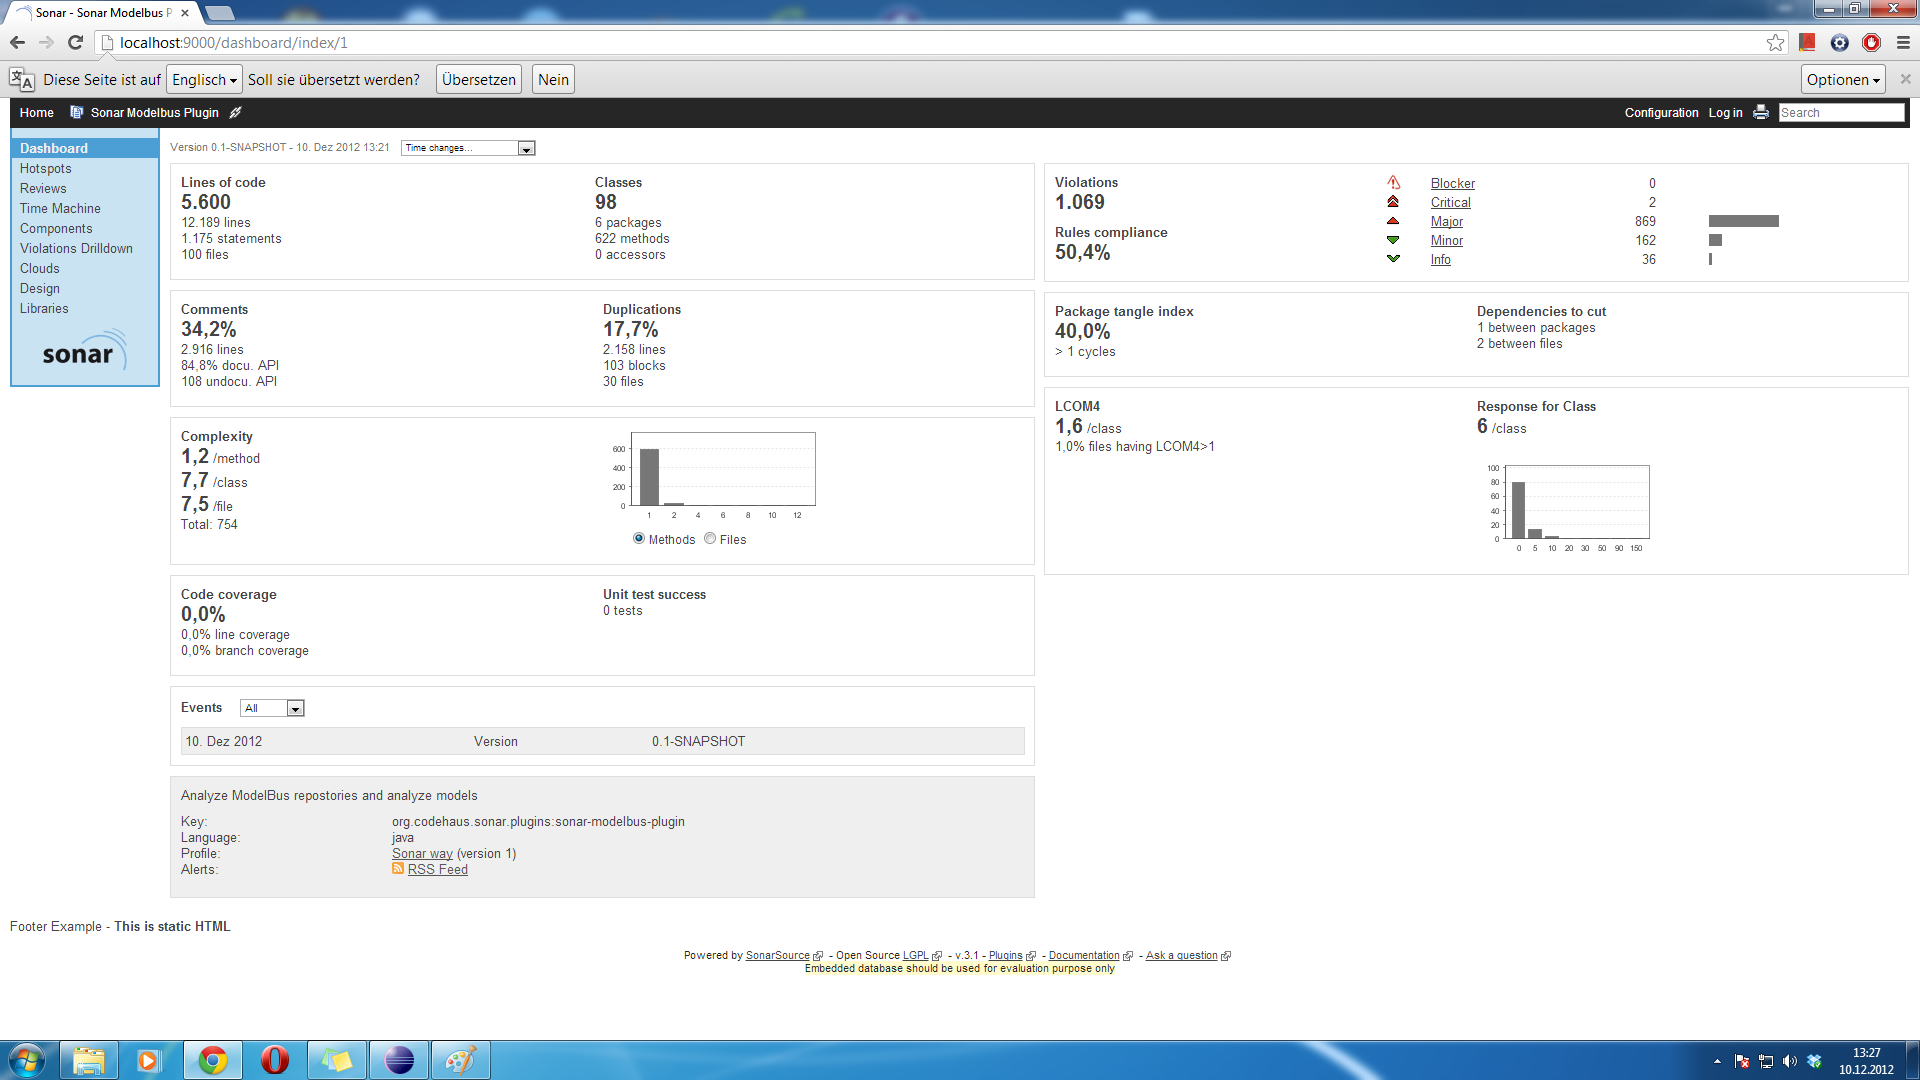
\includegraphics[width=\textwidth]{sonarinaction}
	\caption{Sonar in action}
	\label{fig:sonarinaction}
\end{figure}
\chapter{Conclusion}
\section{Review}
Our opinion about the course ''Softwareproject: Model driven software development'' divides into 2 pieces. The first part tends to an good introduction regarding the content of this seminar. We got basic knowledge about the main content in an enjoyable way and could deploy it a few weeks later. \\
The second part tends to some adverse criticism. The effort of our exercise can be divided into different parts. We really dislike the ratio of the amount of the model driven software development compared to the amount of other tasks. We spend a lot of time to get different things working and developed workarounds because of bugs.  But we required just a few hours to deploy our knowledge of model driven software development to create a smm parser. Therefore, the difficulty is not to use model driven methods, rather than to find an efficient solution of the given task. \\
In addition the whole effort of our task is unpredictable because of Sonar has nearly no documentation. Every technical issue just can be solved with the help of the devlopers mailing list. We think student projects should be a little bit of appreciable.

\section{Conclusion}
Our project was very instructive as well as ordinary. We got an insight of the Frauenhofer Institut what is additionally an gain of knowledge. Within the frame of this course we developed an Sonar plugin that works with Metrino and Modelbus. \\
Because of the leak of time we concentrated our work to developed some basic metrics, just a basic way of visualisation of defined metrics and extended sonar to understand uml. It's possible to enhance our application with additional metrics, more display modes and moreover define more languages like ecore in order that sonar can analyse it. \\ 
It's not a perfect solution but an good example how the given task could be solved and what problems will appear. The classloader problem and other limited functions of the Sonar plugin system are the centre of difficulties. In addition another disadvantage depends the huge build time of an sonar plugin above all if debug mode is activated. For time reasons we couldn't solve one requirement that depends the analyse of real code in the repository. It's not an feature of the current version of sonar and we could not found a workaround but it should be possible in the prospective versions. Furthermore we spend a lot of time in identifying interfaces and comprehend the interaction. This documented knowledge can be used for future works.
\section{Closing Words}
We want to express our appreciation to our course instructor for their effort. We have learned a lot of model driven software development and got an interesting task that intent us the whole time in a positive way. 
\begin{table}
    \begin{tabular}{|l|l|l|l|l|}
        \hline
        Name                                                                    & Start       & Latest end  & Progress & Done by                 \\ \hline
        Explore Modelbus                                                        & Mo 05.11.12 & Fr 09.11.12 & 100%     & Team                    \\ 
        Explore Sonar                                                           & Mo 05.11.12 & Fr 09.11.12 & 100%     & Team                    \\ 
        Explore plugin developement possibilities                               & Mo 05.11.12 & Fr 09.11.12 & 100%     & Ferhat                  \\ 
        Explore Sonar features and developement possibilities                   & Mo 05.11.12 & Fr 09.11.12 & 100%     & Damla                   \\ 
        First attempt to plugin developement                                    & Mo 05.11.12 & Fr 09.11.12 & 100%     & Markus                  \\ 
        Wiki Introduction                                                       & Mo 05.11.12 & Fr 09.11.12 & 100%     & Sebastian               \\ 
        Modelbus connection                                                     & Mo 05.11.12 & Fr 09.11.12 & 100%     & Arsenij                 \\ 
        Sonar documentation                                                     & Mo 05.11.12 & Fr 09.11.12 & 100%     & Markus                  \\ 
        Wiki Metrino                                                            & Mo 05.11.12 & Fr 09.11.12 & 100%     & Alexander               \\ 
        Sonar plugin documentation                                              & Mo 05.11.12 & Fr 09.11.12 & 100%     & Ferhat                  \\ 
        Modelbus documentation                                                  & Mo 05.11.12 & Fr 09.11.12 & 100%     & Damla                   \\ 
        Requirements                                                            & Mo 05.11.12 & Fr 09.11.12 & 100%     & Damla  \&  Ferhat       \\ 
        Presentation Requirements                                               & Mo 05.11.12 & Fr 09.11.12 & 100%     & Ferhat                  \\ 
        Improve requirements                                                    & Mo 12.11.12 & Fr 16.11.12 & 100%     & Damla                   \\ 
        Architecture conecept for sonar                                         & Mo 12.11.12 & Fr 16.11.12 & 100%     & Ferhat                  \\ 
        Architecture conecept for metrino                                       & Mo 12.11.12 & Fr 16.11.12 & 100%     & Alexander               \\ 
        Introduction to wiki                                                    & Mo 12.11.12 & Mo 19.11.12 & 100%     & Sebastian               \\ 
        Presentation Template                                                   & Mo 12.11.12 & Fr 19.11.12 & 100%     & Damla                   \\ 
        Software architecture – sequencediagram/activitydiagram                 & Mo 12.11.12 & Fr 23.11.12 & 100%     & Sebastian               \\ 
        Setup Modelbus Repository Server                                        & Mo 19.11.12 & Mo 26.11.12 & 100%     & Arsenij                 \\ 
        Explore howto running sonar on a repository                             & Di 20.11.12 & Mo 26.11.12 & 100%     & Arsenij                 \\ 
        Installation of software components                                     & Do 23.11.12 & Do 23.11.12 & 100%     & Team                    \\ 
        Example Sonar plugin                                                    & Mo 19.11.12 & Fr 23.11.12 & 100%     & Unknown                 \\ 
        Multilanguage(different programming languages) support in sonar plugins & Fr 23.11.12 & Do 29.11.12 & 100%     & Markus  \&  Damla  \&  Ferhat \\ 
        Sequence diagram for the work of sonar with Metrino and ModelBus        & So 25.11.12 & So 25.11.12 & 100%     & Damla  \&  Sebastian    \\ 
        Setup modelbus server                                                   & Fr 23.11.12 & Mo 26.11.12 & 100%     & Markus                  \\ 
        Presentation first architecture                                         & Fr 23.11.12 & Mo 26.11.12 & 100%     & Ferhat                  \\ 
        Activity diagram modelbus repository                                    & Fr 23.11.12 & Mo 26.11.12 & 100%     & Damla                   \\ 
        SOAP Client Metrino                                                     & Fr 23.11.12 & Do 06.12.12 & 100%     & Alexander               \\ 
        Wiki Logo and header                                                    & Mo 26.11.12 & Fr 30.11.12 & 100%     & Ferhat                  \\ 
        OCL  \&  Documentation                                                  & Mo 26.11.12 & Fr 30.11.12 & 100%     & Damla  \&  Ferhat       \\ 
        Milestone definitions and description                                   & Mo 26.11.12 & Fr 30.11.12 & 100%     & Sebastian               \\ 
        Installation manual                                                     & Mo 03.12.12 & Mo 10.12.12 & 100%     & Sebastian               \\ 
        Include other language plugins with modules                             & Mo 03.12.12 & Mo 10.12.12 & 100%     & Arsenij                 \\ 
        Client without using WSDL by hand                                       & Mo 03.12.12 & Mo 10.12.12 & 100%     & Markus                  \\ 
        Objectoriented Analysis to Models                                       & Mo 03.12.12 & Mo 10.12.12 & 100%     & Ferhat                  \\ 
        Understand Metrino metrcis                                              & Mo 10.12.12 & Fr 21.12.12 & 100%     & Sebastian  \&  Alexander \\ 
        ownload modelbus files in a sonar plugin                                & Mo 10.12.12 & Fr 21.12.12 & 100%     & Markus                  \\ 
        Create latex documentation                                              & Mo 17.12.12 & Fr 21.12.12 & 100%     & Ferhat                  \\ 
        Meeting Protocols to latex documentation                                & Mo 17.12.12 & Fr 21.12.12 & 100%     & Damla                   \\ 
        Metrino CheckModel, download and parse SMM from Repo                    & Mo 07.01.13 & Mo 21.01.13 & 100%     & Arsenij                 \\ 
        Sonar frontend                                                          & Mo 07.01.13 & Mo 21.01.13 & 100%     & Sebastian               \\ 
        Parser for SMM                                                          & Mo 14.01.13 & So 20.01.13 & 100%     & Damla  \&  Ferhat       \\ 
        Using of EMF to parse SMM files                                         & Mo 21.01.13 & Mo 28.01.13 & 100%     & Damla  \&  Ferhat       \\ 
        Include parser into project workflow                                    & Mo 21.01.13 & Mo 28.01.13 & 100%     & Damla  \&  Ferhat       \\ 
        Merge all components into one                                           & Mo 21.01.13 & Mo 28.01.13 & 100%     & Arsenij                 \\ 
        Project spezific measurements in sonar                                  & Mo 21.01.13 & Mo 28.01.13 & 100%     & Markus                  \\ 
        ceate ocl metrics                                                       & Mo 21.01.13 & So 03.02.13 & 100%     & Alexander               \\ 
        Color Measurements                                                      & Mo 21.01.13 & Mo 28.01.13 & 100%     & Sebastian               \\ 
        Documentation in Latex                                                  & Mo 28.01.13 & Mo 18.02.13 & 25%      & Team                    \\ 
        SMM Adapter                                                             & Mo 28.01.13 & Mo 18.02.13 & 67%      & Arsenij                 \\ 
        Load dynamic metrics in sonar                                           & Mo 28.01.13 & Mo 18.02.13 & 36%      & Sebastian               \\ 
        Meeting Protocols                                                       & Mo 03.12.12 & Mo 18.02.13 & 95%      & Damla  \&  Ferhat       \\ 
        ~                                                                       & ~           & ~           & ~        & ~                       \\ 
        ~                                                                       & ~           & ~           & ~        & ~                       \\ 
        ~                                                                       & ~           & ~           & ~        & ~                       \\ 
        ~                                                                       & ~           & ~           & ~        & ~                       \\ 
        ~                                                                       & ~           & ~           & ~        & ~                       \\ 
        ~                                                                       & ~           & ~           & ~        & ~                       \\
        \hline
    \end{tabular}
\end{table}
\end{document}
